\documentclass[a4paper,oneside,fleqn,titlepage]{book}
\usepackage[T1]{fontenc}
\usepackage[utf8]{inputenc}
\usepackage[italian]{babel}

%%%%% Pacchetti caricati
\usepackage{fancyhdr}
\usepackage{layaureo}
\usepackage[font=small,format=hang,labelfont=bf,textformat=period]{caption}
% per tabelle e figure
\usepackage{booktabs,graphicx,subfig}
\usepackage{tikz,tikz-3dplot}
\usepackage[autostyle=true]{csquotes}
\usepackage[style=mythesis,hyperref,abbreviate=false,backend=biber]{biblatex}
\usepackage{listings}
% `listingsutf8' serve per risolvere il problema di `listings' con gli
% accenti. Per un workaround alternativo vedi il sito
% http://stackoverflow.com/questions/1116266/
\usepackage{listingsutf8}
% `mathtools' serve per definire la norma e il valore assoluto
\usepackage{mathtools}
\usepackage{frontespizio}
\usepackage{amsmath,amsfonts,amssymb,amsthm}
% `bm' serve per scrivere i vettori in corsivo con il comando
% `\bm{vettore}'. Deve sostituire il comando `\mathbf{vettore}' perché questo
% restituisce erroneamente lettere in tondo, non in corsivo e non funziona con
% le lettere greche.
\usepackage{bm}
\usepackage{siunitx}
\usepackage{hyperref}
%%%%% Fine pacchetti

%%%%% Impostazioni
%% testatine.
% TODO: decidere se usare `oneside' o `twoside' e adattare il formato della
% testatina di conseguenza.
\pagestyle{fancy}
\fancyhf{} % svuota tutti i campi delle testatine e dei piedi
% Abbiamo usato l'opzione di classe `oneside', quindi la testatina è la stessa
% per tutte le pagine.
% Nella testatina (`head') a destra (`R') mettiamo il nome del paragrafo
% (`\rightmark'), non tutto maiuscolo (`\nouppercase').
\fancyhead[R]{\slshape\footnotesize\nouppercase{\leftmark}}
% Nel piede (`foot') al centro (`C') mettiamo il numero della pagina
% (`\thepage').
\fancyfoot[C]{\thepage}

\graphicspath{{Immagini/}} % cartella in cui cercare le immagini da caricare

% impostazioni per il pacchetto `hyperref'. Per l'elenco di tutte le opzioni del
% documento consulta il manuale: `texdoc hyperref'
\hypersetup{pdftitle={Problema dei due corpi e applicazioni astrofisiche},
  colorlinks,% link colorati, non riquadrati
  breaklinks=true,% permette di spezzare i link su più righi
  bookmarksnumbered,% inserisce i numeri delle sezioni nei segnalibri
  urlcolor=black,linkcolor=black,citecolor=black
}

\sisetup{per-mode=symbol,
  inter-unit-separator={}\cdot{},
  exponent-product=\cdot,
  output-product=\cdot,
  separate-uncertainty=true
}

% Posiziona le didascalie sopra le tabelle
\captionsetup[table]{position=top}

%% Nuove unità di misura
\DeclareSIUnit\parsec{pc}
\DeclareSIUnit\year{yr}
\DeclareSIUnit\solarmass{\ensuremath{M_\odot}}
% C'era già l'arcosecondo, però lo ridefinisco per essere coerente con gli
% articoli che cito
\DeclareSIUnit\arcsecond{as}

\bibliography{bibliografia} % nome del file contenente la bibliografia
\defbibheading{subbibliography}{\section*{#1}\markboth{#1}{#1}}

\theoremstyle{plain}
\newtheorem*{teorema}{Teorema}

% impostazioni del pacchetto `listings'.
\lstset{basicstyle=\small\ttfamily,showstringspaces=false,frame=lines,
  numbers=left,numberstyle=\tiny,extendedchars=true,inputencoding=utf8/latin1}

\addto\captionsitalian{%
  \renewcommand{\lstlistingname}{Codice}}

\usetikzlibrary{calc,intersections}
%%%%% Fine impostazioni

%%%%% Comandi personalizzati
% ridefinisco i comandi per alcune lettere greche in modo che si usino le
% varianti
\renewcommand{\phi}{\varphi}
\renewcommand{\epsilon}{\varepsilon}

% Operatori
\newcommand*{\dd}{\mathop{}\!\mathrm{d}} % Operatore differenziale \dd
\DeclareMathOperator{\uimm}{\mathrm{i}} % unità immaginaria
% Operatore valore assoluto \abs{x}. Usa \abs*{} per le frazioni
\DeclarePairedDelimiter{\abs}{\lvert}{\rvert}
% Operatore norma \norm{x}. Usa \norm*{} per le frazioni
\DeclarePairedDelimiter{\norm}{\lVert}{\rVert}

%% Derivate
% Derivata totale: \toder[ordine]{funzione}{variabile}
\newcommand*{\toder}[3][]{\frac{{\dd^{#1}}#2}{\dd {#3}^{#1}}}
% Derivata parziale \parder[ordine]{funzione}{variabile}
% Per la definizione del comando `parder' (per inserire le derivate parziali)
% vedi http://www.guit.sssup.it/phpbb/viewtopic.php?p=42188#42188
\makeatletter
\newcommand{\parder}[2]{\begingroup
  \@tempswafalse\toks@={}\count@=\z@
  \@for\next:=#2\do
    {\expandafter\check@var\next\@nil
     \advance\count@\parder@exp
     \if@tempswa
       \toks@=\expandafter{\the\toks@\,}%
     \else
       \@tempswatrue
     \fi
     \toks@=\expandafter{\the\expandafter\toks@\expandafter\partial\parder@var}}%
  \frac{\partial\ifnum\count@=\@ne\else^{\number\count@}\fi#1}{\the\toks@}%
  \endgroup}
\def\check@var{\@ifstar{\mult@var}{\one@var}}
\def\mult@var#1#2\@nil{\def\parder@var{#2^{#1}}\def\parder@exp{#1}}
\def\one@var#1\@nil{\def\parder@var{#1}\chardef\parder@exp\@ne}
\makeatother

% Derivate per le formule in linea (usare \frac in linea è eccessivo). La `l'
% iniziale nel nome distingue questi comandi da quelli per le formule fuori
% corpo. Non uso `\dd' ma `\mathrm{d}' perché nelle formule in linea `\dd'
% aggiunge una spaziatura non adatta. Non sono dei comandi bellissimi, ma
% permettono di passare facilmente da formula in linea a fuori corpo e viceversa
% cambiando una lettera.
% Derivata totale: \ltoder[ordine]{funzione}{variabile}
\newcommand*{\ltoder}[3][]{\mathrm{d}^{#1}#2 / \mathrm{d} {#3}^{#1}}
% Derivata parziale: \lparder[ordine]{funzione}{variabile}
\newcommand*{\lparder}[3][]{\partial^{#1} #2 / \partial {#3}^{#1}}
% NOTA: `\parder' e `\lparder' non sono completamente interscambiabili, il primo
% comando è molto più complesso e permette di inserire le derivate miste, a
% differenza del secondo.

% Costante di Eulero
\DeclareMathOperator{\e}{\mathrm{e}}
% Versore. Esempi: versore x: `\versore{x}', versore i: \versor{\imath}, versore
% j: \versor{\jmath} (solo `i' e `j' richiedono `\imath' e `\jmath', altrimenti
% il puntino litiga con `\hat')
\newcommand*{\versor}[1]{\hat{\bm{#1}}}

% Ambiente per scrivere sistemi di equazioni.
% Vedi `L'arte di scrivere con LaTeX' di Pantieri.
% Esempio d'uso (in ambiente matematico):
%	\begin{sistema}
%         x+y+z=0 \\
%         2x-y=1 \\
%         y-4z=-3
%       \end{sistema}
\newenvironment{sistema}%
{\left\lbrace\begin{array}{@{}l@{}}}%
    {\end{array}\right.}

%% Campi notevoli
\let\numberset\mathbb
\newcommand{\Z}{\numberset{Z}}	% Interi \Z
\newcommand{\R}{\numberset{R}}	% Reali \R
\newcommand{\C}{\numberset{C}}	% Complessi \C
%%%%% Fine comandi personalizzati

%%%%% Funzioni PGF
% funzione che restituisce la distanza dal fuoco di un punto di un'ellisse in
% corrispondenza dell'anomalia vera #1 (\e = eccentricità, \p = semilato retto)
\pgfmathdeclarefunction{dist}{1}{\pgfmathparse{\p/(1+\e*cos(#1))}}
% vedi equazione (1.51), pag 10 della tesi (eq:angolo-alpha2). Per avere
% risultati corretti bisogna inserire un valore dell'anomalia diverso da 0,
% 180 e 360 (e numeri a loro congrui in modulo 360)
\pgfmathdeclarefunction{alpha}{1}{\pgfmathparse{
    (mod(#1,360) < 180) ? atan(1/tan(mod(#1,360))+1/(\e*sin(mod(#1,360)))):
                          atan(1/tan(mod(#1,360)) +
                          1/(\e*sin(mod(#1,360)))) + 180}
}
% vedi sempre il paragrafo sulla velocità nella direzione della linea di
% vista (sec:velocita-linea-di-vista)
\pgfmathdeclarefunction{beta}{1}{\pgfmathparse{#1+alpha(#1)}}
%%%%% Fine funzioni PGF

\begin{document}
\frontmatter{}
\pagenumbering{Alph}
\begin{frontespizio}
\Istituzione{Università degli Studi del Salento}
\Logo{Immagini/logo_unisalento}
\Facolta{Scienze Matematiche Fisiche e Naturali}
\Corso[Laurea triennale]{Fisica}
\Annoaccademico{2010--2011}
\Titoletto{Tesi di Laurea}
\Titolo{Il problema dei due corpi\\
  e applicazioni astrofisiche}
\Candidato{Mosè Giordano}
\Relatore{Dott. Achille Nucita}
\end{frontespizio}

%%% Local Variables:
%%% mode: latex
%%% TeX-master: "tesi"
%%% End:


\clearpage{}
\pagenumbering{roman}
\tableofcontents{}
\clearpage{}
\listoffigures{}

\mainmatter{}
\chapter{Il problema dei due corpi}
\label{chap:due-corpi}

In questo capitolo affronteremo il \emph{problema dei due corpi}, cioè lo studio
del moto di due corpi, supposti puntiformi, soggetti solamente alla mutua
interazione dovuta a forze che soddisfano il principio di azione e reazione. In
particolare ci occuperemo del \emph{problema di Keplero}, ovvero del caso in cui
la forza fra i due corpi è quella gravitazionale, che è di tipo centrale. Il
problema sarà risolto usando il formalismo newtoniano (si vedano
\textcites{bradt:processes}{fabrizio:meccanica}{smart:textbook}) e quelli
lagrangiano e hamiltoniano (si vedano
\textcites{goldstein:meccanica}{landau:meccanica}), di questi ultimi daremo una
breve presentazione. Riusciremo a determinare analiticamente le equazioni delle
orbite dei due corpi e a dedurre alcune proprietà del sistema. La risoluzione
del problema di Keplero permette di descrivere, fra le altre cose, il moto di
due corpi celesti, per esempio un pianeta e la sua stella, che sono soggetti
solo alla mutua interazione gravitazionale.

\section{Formalismo newtoniano}
\label{sec:formalismo-newton}

\begin{figure}
  \centering
  \begin{tikzpicture}[font=\footnotesize,scale=3]
    % m1=1: y=0.8,  z=0.2,  x=0.2
    % m2=3: y=0.6,  z=0.8,  x=0.4
    % cm:   y=0.65, z=0.65, x=0.35
    \node [shape=coordinate](O) at (0,0,0) [label=left:$O$] {};
    \draw [->] (O) -- (1,0,0) node[right] {$y$}; % asse y
    \draw [->] (O) -- (0,1,0) node[above] {$z$}; % asse z
    \draw [->] (O) -- (0,0,1) node[below left] {$x$}; % asse x
    \filldraw [gray] (0.8,0.2,0.2) circle (0.01); % corpo di massa m_2
    \draw [->] (0,0,0) -- node[below right,fill=white] {$\bm{r}_2$}
               (0.8,0.2,0.2) node[right] {$m_2$}; % vettore r_2
    \filldraw [gray] (0.6,0.8,0.4) circle (0.02); % corpo di massa m_1
    \draw [->] (0,0,0) -- node[above left] {$\bm{r}_1$} (0.6,0.8,0.4)
               node[above] {$m_1$}; % vettore r_1
    % vettore posizione relativa
    \draw [<-] (0.8,0.2,0.2) -- node[right] {$\bm{r}$} (0.6,0.8,0.4);
    % vettore posizione del centro di massa
    \draw [->] (0,0,0) -- node[right] {$\bm{r}_\textup{CM}$} (0.65,0.65,0.35);
  \end{tikzpicture}
  \caption{Due corpi in un sistema di riferimento inerziale}
  \label{fig:due-corpi}
\end{figure}
Consideriamo un sistema costituito da due corpi puntiformi, di masse $m_1$ e
$m_2$ e in un fissato sistema di riferimento inerziale indichiamo con $\bm{r}_1$
e $\bm{r}_2$ i rispettivi vettori posizione, come nella
Figura~\ref{fig:due-corpi}. Per la seconda legge di Newton, la forza
$\bm{F}_{21}$ che il corpo di massa $m_1$ esercita sul corpo di massa $m_2$ è
data da
\begin{equation}
  \label{eq:f21}
  \bm{F}_{21} = m_2\toder[2]{\bm{r}_2}{t}
\end{equation}
e la forza $\bm{F}_{12}$ che il corpo di massa $m_2$ esercita sull'altro è
\begin{equation}
  \label{eq:f12}
  \bm{F}_{12} = m_1\toder[2]{\bm{r}_1}{t}.
\end{equation}
Assumiamo per ipotesi che queste due forze soddisfino il principio di azione e
reazione nella forma forte (si veda \textcite{goldstein:meccanica})
\begin{equation}
  \label{eq:azione-reazione}
  \bm{F}_{12} = -\bm{F}_{21}.
\end{equation}
Definiamo il vettore \emph{posizione relativa}
\begin{equation}
  \label{eq:posizione-relativa}
  \bm{r}=\bm{r}_2-\bm{r}_1
\end{equation}
e il vettore posizione del \emph{centro di massa}
\begin{equation}
  \label{eq:centro-di-massa}
  \bm{r}_\textup{CM} = \frac{m_1\bm{r}_1+m_2\bm{r}_2}{m_1+m_2}.
\end{equation}
Dalle equazioni~\eqref{eq:posizione-relativa} e~\eqref{eq:centro-di-massa}
possiamo ricavare $\bm{r}_1$ e $\bm{r}_2$ in funzione di $\bm{r}$ e
$\bm{r}_\textup{CM}$
\begin{subequations}
  \label{eq:r1-r2-posizione-relativa-cdm}
  \begin{align}
    \bm{r}_1 &= \bm{r}_\textup{CM} - \frac{m_2}{m_1+m_2}\bm{r} =
    \bm{r}_\textup{CM} - \frac{\mu}{m_1}\bm{r},\\
    \bm{r}_2 &= \bm{r}_\textup{CM} + \frac{m_1}{m_1+m_2}\bm{r} =
    \bm{r}_\textup{CM} + \frac{\mu}{m_2}\bm{r},
  \end{align}
\end{subequations}
in cui abbiamo introdotto la \emph{massa ridotta} $\mu$ definita dalla metà
della media armonica fra $m_1$ e $m_2$
\begin{equation}
  \frac{1}{\mu} = \frac{1}{m_1} + \frac{1}{m_2} \iff \mu=\frac{m_1m_2}{m_1+m_2}.
\end{equation}
Osserviamo che la massa ridotta è sempre minore delle due masse, infatti
\begin{equation}
  \mu =\frac{m_1}{m_1/m_2+1} = \frac{m_2}{1+m_2/m_1},
\end{equation}
quindi $\mu < m_1,m_2$ per qualsiasi valore positivo delle due masse. Definiamo
inoltre la \emph{massa totale} $M_\textup{T}$ del sistema
\begin{equation}
  M_\textup{T}=m_1+m_2.
\end{equation}
Dalle definizioni di massa ridotta e totale deriva che
$M_\textup{T}\mu=m_1m_2$. Se, per esempio, $m_1\gg m_2$, allora $\mu\simeq m_2$ e
$M_\textup{T}\simeq m_1$. L'equazione del moto del centro di massa può essere
trovata semplicemente calcolando l'accelerazione di $\bm{r}_\textup{CM}$
\begin{equation}
  \toder[2]{\bm{r}_\textup{CM}}{t} = \frac{1}{M_\textup{T}}
  \left(
    m_1\toder[2]{\bm{r}_1}{t} + m_2\toder[2]{\bm{r}_2}{t}
  \right) = \frac{\bm{F}_{12}+\bm{F}_{21}}{M_\textup{T}} = \bm{0},
\end{equation}
cioè il centro di massa è in quiete o si muove di moto rettilineo
uniforme. Consideriamo, quindi, come sistema di riferimento inerziale quello
avente origine nel centro di massa. In questo nuovo sistema le posizioni delle
due masse saranno dunque descritte dai vettori
\begin{subequations}
  \label{eq:r1-r2-nel-cdm}
  \begin{align}
    \bm{r}_1 &= -\frac{\mu}{m_1}\bm{r}, \label{eq:r1-nel-cdm}\\
    \bm{r}_2 &= \frac{\mu}{m_2}\bm{r}.
  \end{align}
\end{subequations}
Osserviamo che se, per esempio, $m_1\gg m_2$, allora $\bm{r}_1\simeq\bm{0}$,
cioè il corpo più massivo si trova praticamente nel centro di massa, come è
logico aspettarsi dalla definizione di centro di massa.

Dividendo ambo i membri della~\eqref{eq:f21} per $m_2$, ambo i membri
della~\eqref{eq:f12} per $m_1$ e sottraendo membro a membro le equazioni così
ottenute ricaviamo
\begin{equation}
  \frac{\bm{F}_{21}}{m_2}-\frac{\bm{F}_{12}}{m_1} = \bm{F}_{21}
  \left(
    \frac{1}{m_2}+\frac{1}{m_1}
  \right) = \frac{\bm{F}_{21}}{\mu} = \toder[2]{(\bm{r}_2-\bm{r}_1)}{t} =
  \toder[2]{\bm{r}}{t}
\end{equation}
in cui abbiamo ricordato che vale il principio di azione e reazione espresso
dalla~\eqref{eq:azione-reazione}. L'equazione precedente può essere riscritta
nella forma
\begin{equation}
  \label{eq:f21-mu}
  \bm{F}_{21}=\mu\toder[2]{\bm{r}}{t}
\end{equation}
da cui possiamo dedurre che il problema del moto relativo dei due corpi si è
ridotto allo studio del moto di un solo corpo fittizio, che chiameremo
\emph{particella relativa}, di massa $\mu$ all'interno del campo generato da un
altro corpo fittizio puntiforme di massa $M_\textup{T}$ e fisso, istante per
istante, nella posizione di uno dei due corpi. Poiché nel nostro caso abbiamo
definito la posizione relativa come $\bm{r}=\bm{r}_2 - \bm{r}_1$, abbiamo che il
corpo fittizio di massa pari alla massa totale occupa la posizione del corpo
reale di massa $m_1$. Istante per istante il vettore $\bm{r}$ indica la
posizione della particella fittizia $\mu$ nel sistema di riferimento di
$M_\textup{T}$.

\subsection{Problema di Keplero}
\label{sec:problema-keplero}

Consideriamo il caso dell'interazione gravitazionale. Se indichiamo con $M$ la
massa del corpo che genera il campo a cui è soggetto un corpo di massa $m$ e con
$\bm{r}$ il vettore diretto dal corpo di massa $M$ verso il corpo di massa $m$,
allora la forza $\bm{F}_\textup{G}$ agente su $m$ è data da
\begin{equation}
  \label{eq:legge-attrazione}
  \bm{F}_\textup{G} = -\frac{GMm}{r^2}\versor{r},
\end{equation}
in cui $G=\SI{6.673 84(80)e-11}{\cubic\metre\per\kilogram\per\second\squared}$ è
la costante di gravitazione universale (il valore della costante è preso da
\textcite{codata:costanti}). Si tratta di una forza centrale, cioè puramente
radiale, e il segno meno indica che è sempre attrattiva verso il centro del
campo. Sostituendo la~\eqref{eq:legge-attrazione} nella~\eqref{eq:f21-mu}
abbiamo
\begin{equation}
  \label{eq:forza-mu}
  \bm{F}_{21} = -\frac{GM_\textup{T}\mu}{r^2}\versor{r} =
  -\frac{Gm_1m_2}{r^2}\versor{r} = \mu\toder[2]{\bm{r}}{t}.
\end{equation}

Per una qualsiasi forza di tipo centrale il momento angolare $\bm{l} = \bm{r}
\times \bm{p}$ rispetto al centro della forza è una costante del moto. Infatti
il momento torcente $\bm{\tau}$ di una forza $\bm{F}$ rispetto a un polo $O$ è
definito da
\begin{equation}
  \bm{\tau}= \toder{\bm{l}}{t} = \bm{r}\times\bm{F}.
\end{equation}
Qui con $\bm{r}$ indichiamo il vettore congiungente il polo con il punto di
applicazione della forza. Poiché la forza $\bm{F}$ è radiale, il momento
torcente associato è nullo, implicando quindi la costanza nel tempo del momento
angolare $\bm{l}$ calcolato rispetto allo stesso polo.

Ritornando al problema di Keplero, abbiamo appena visto che il momento angolare
della particella di massa ridotta rispetto alla posizione di $M_\textup{T}$ è un
integrale primo del moto. Notiamo ora che, per definizione di momento angolare,
i vettori $\bm{r}$ e $\bm{l}\equiv\bm{l}_0$ sono fra loro perpendicolari. Allora
la costanza del vettore $\bm{l}_0$, e in particolare della sua direzione,
implica che, nel caso $\bm{l}_0\neq\bm{0}$, il vettore $\bm{r}$, giace sempre
sullo stesso piano perpendicolare a $\bm{l}_0$. Se invece risulta
$\bm{l}_0=\bm{0}$, $\bm{r}$ è parallelo alla quantità di moto $\bm{p}$ e il moto
è unidimensionale. Da qui in seguito supporremo che il momento angolare
$\bm{l}_0$ della particella relativa sia non nullo.

Dal momento che il moto della particella di massa ridotta si svolge in un piano,
possiamo utilizzare le coordinate polari $r,\theta$ per rappresentare la
posizione del corpo nel sistema di riferimento di $M_\textup{T}$. Dalla
meccanica si ricava che per un moto piano la velocità $\dot{\bm{r}}$ e
l'accelerazione $\ddot{\bm{r}}$ del vettore posizione $\bm{r}=r\versor{r}$ sono
date da
\begin{subequations}
  \begin{align}
    \dot{\bm{r}}  &= \dot{r}\versor{r} +
    r\dot{\theta}\versor{\theta}, \label{eq:velocita-polare}\\
    \ddot{\bm{r}} &= (\ddot{r}-r\dot{\theta}^2)\versor{r} + (r\ddot{\theta} +
    2\dot{r}\dot{\theta}) \versor{\theta}.
  \end{align}
\end{subequations}
Usando le coordinate polari, l'equazione vettoriale~\eqref{eq:forza-mu} può
essere riscritta come due equazioni scalari
\begin{subequations}
  \begin{gather}
    -\frac{GM_\textup{T}\mu}{r^2} = \mu(\ddot{r} - r\dot{\theta}^2) \iff
    -\frac{GM_\textup{T}}{r^2}=\ddot{r}-r\dot{\theta}^2,
    \label{eq:forza-mu-radiale}\\
    0 = \mu(r\ddot{\theta} +
    2\dot{r}\dot{\theta}). \label{eq:forza-mu-azimutale}
  \end{gather}
\end{subequations}
Dalla~\eqref{eq:forza-mu-azimutale} si trova nuovamente la costanza del modulo
$l_0 = \norm{\bm{l}_0} = \mu r^2\dot{\theta}$ del momento angolare. Infatti
\begin{equation}
  0 = r\mu(r\ddot{\theta} + 2\dot{r}\dot{\theta}) = \toder{\mu
    r^2\dot{\theta}}{t} = \toder{l_0}{t}.
\end{equation}

\begin{figure}
  \centering
  \begin{tikzpicture}[font=\footnotesize,scale=2]
    \draw[->] (0.6,1.2) .. controls (0.8,1.19) and (1.1,1.196) .. (1.299,0.75)
                        .. controls (1.5,0.3)  and (1.7,0.2)   .. (2.0,0.0)
                        .. controls (2.3,-0.2) and (2.4,-0.2)  .. (2.6,-0.3);
    \draw (0,0) node[left] {$O$};
    \draw[->] (0,0) -- node[below] {$r+\dd r$} (2,0);
    \draw[->] (0,0) -- node[above] {$r$} (1.299,0.75);
    \draw[dashed] (1.299,0) -- node[left] {$r\dd\theta$} (1.299,0.75);
    \draw[->] ($0.4*cos(30)*(1,0)+ 0.4*sin(30)*(0,1)$) to [out=-60,in=90]
              node[right] {$\dd\theta$} (0.4,0);
  \end{tikzpicture}
  \caption[Area spazzata nell'intervallo di tempo $\dd t$ dal vettore
  posizione]{Area spazzata nell'intervallo di tempo $\dd t$ dal vettore
    posizione di un corpo in moto lungo una traiettoria generica}
\label{fig:area-differenziale}
\end{figure}
L'area differenziale $\dd A$ spazzata dalla particella di massa ridotta che si
sposta di un angolo infinitesimo $\dd\theta$ è espressa da (si veda la
Figura~\ref{fig:area-differenziale})
\begin{equation}
  \dd A = \frac{r\cdot r\dd\theta}{2} = \frac{r^2\dd\theta}{2},
\end{equation}
quindi la velocità areolare $\ltoder{A}{t}$ è
\begin{equation}
  \label{eq:velocita-areolare}
  \toder{A}{t} = \frac{1}{2}r^2\dot{\theta} = \frac{1}{2}\frac{l_0}{\mu} =
  \text{costante}.
\end{equation}
Abbiamo così ottenuto la seconda legge di Keplero:
\textbf{\emph{il vettore posizione della particella rispetto al centro
    dell'orbita (o della forza) spazza aree uguali in intervalli di tempo
    uguali}}. Osserviamo che per giungere a questo risultato è stato sufficiente
utilizzare la costanza del momento angolare che deriva a sua volta dal carattere
centrale della forza; pertanto questa legge è valida per tutte le forze di
questo tipo.

\subsection{Equazione dell'orbita}
\label{sec:equazione-dellorbita}

Nel problema di Keplero, vogliamo ora cercare un'espressione esplicita della
coordinata polare $r$ in funzione dell'altra coordinata $\theta$, che a sua
volta dipenderà dal tempo. Per fare ciò è conveniente effettuare la sostituzione
$u=1/r$. Calcolando le derivate temporali di $r$ otteniamo che
\begin{subequations}
  \begin{align}
    \dot{r} &= \toder{r}{t} = \toder{r}{\theta}\toder{\theta}{t} =
    \toder{(1/u)}{\theta}\dot{\theta} =
    -\frac{\dot{\theta}}{u^2}\toder{u}{\theta}
    = -\frac{l_0}{\mu}\toder{u}{\theta}, \label{eq:derivata1-r}\\
    \begin{split}
      \ddot{r} &= \toder[2]{r}{t} = \toder{}{\theta}
      \left( \toder{r}{t} \right)\toder{\theta}{t} = \toder{}{\theta}
      \left( -\frac{l_0}{\mu}\toder{u}{\theta} \right)\dot{\theta} =
      -\frac{l_0\dot{\theta}}{\mu}\toder[2]{u}{\theta} \\
      &= - \left( \frac{l_0}{\mu}
      \right)^2u^2\toder[2]{u}{\theta}. \label{eq:derivata2-r}
    \end{split}
  \end{align}
\end{subequations}
Sostituendo la~\eqref{eq:derivata2-r} nella~\eqref{eq:forza-mu-radiale} abbiamo
\begin{equation}
  -GM_\textup{T}u^2 = -
  \left(
    \frac{l_0}{\mu}
  \right)^2u^2\toder[2]{u}{\theta} - \frac{l_0^2u^3}{\mu^2}.
\end{equation}
Poiché $r$ rappresenta la distanza della particella di massa ridotta da
$M_\textup{T}$, essa assume valori finiti e il suo reciproco $u$ non è mai
nullo. Nell'equazione precedente possiamo quindi dividere ambo i membri per
$u^2$ ottenendo
\begin{equation}
  \toder[2]{u}{\theta} + u = \frac{GM_\textup{T}\mu^2}{l_0^2}.
\end{equation}
Questa è una equazione differenziale ordinaria lineare del secondo ordine a
coefficienti costanti, chiamata \emph{equazione di Binet}
(si veda \textcite{fabrizio:meccanica}). Per semplificare i calcoli poniamo
\begin{equation}
  \label{eq:reciproco-semilato}
  \frac{GM_\textup{T}\mu^2}{l_0^2} = \frac{1}{p},
\end{equation}
di modo che l'integrale generale dell'equazione di Binet diventa
\begin{equation}
  \label{eq:soluzione-binet}
  u(\theta) = c_0\cos\theta + c_1\sin\theta + \frac{1}{p},
\end{equation}
con $c_0$ e $c_1$ costanti di integrazione. Imponiamo le seguenti condizioni
iniziali
\begin{subequations}
  \label{eq:condizioni-binet}
  \begin{align}
    u(\theta_0) &= \frac{1+e}{p},\\
    \toder{u}{\theta}(\theta_0) &= 0,
  \end{align}
\end{subequations}
che significano richiedere che il punto $\theta = \theta_0$ sia stazionario per
la funzione $u(\theta)$ e che in questo punto la funzione $u$ assuma il valore
$(1+e)/p$. Vedremo più avanti il significato delle grandezze $e$ e
$p$. Osserviamo che queste condizioni equivalgono a richiedere
\begin{subequations}
  \begin{align}
    r(\theta_0) &= \frac{1}{u(\theta)} = \frac{p}{1+e}, \\
    \toder{r}{\theta}(\theta_0) &= \toder{(1/u)}{\theta}(\theta_0) =
    -\frac{1}{u^2(\theta_0)} \toder{u}{\theta}(\theta_0) = 0.
  \end{align}
\end{subequations}
Con le condizioni~\eqref{eq:condizioni-binet} le costanti di integrazione
valgono
\begin{subequations}
  \label{eq:costanti-binet}
  \begin{align}
    c_0 &= \frac{e}{p}\cos\theta_0, \\
    c_1 &= \frac{e}{p}\sin\theta_0,
  \end{align}
\end{subequations}
pertanto la soluzione dell'equazione di Binet~\eqref{eq:soluzione-binet} con le
condizioni~\eqref{eq:condizioni-binet} è
\begin{equation}
  \label{eq:soluzione2-binet}
  u(\theta) = \frac{1}{p}(1 + e\cos\theta\cos\theta_0 +
  e\sin\theta\sin\theta_0) =  \frac{1}{p}(1+e\cos(\theta-\theta_0)).
\end{equation}
Ricordando che $r(\theta)=1/u(\theta)$ giungiamo, infine, all'equazione polare
dell'orbita della particella relativa nel sistema di riferimento di
$M_\textup{T}$
\begin{equation}
  \label{eq:orbita}
  r(\theta) = \frac{p}{1+e\cos(\theta-\theta_0)}.
\end{equation}

\subsection{Classificazione geometrica delle orbite}
\label{sec:class-geom-orbite}

La~\eqref{eq:orbita} è l'equazione polare di una conica con centro nel fuoco o
uno dei fuochi nel caso dell'ellisse. La costante $e$ è chiamata
\emph{eccentricità} della conica, la costante $p$ invece è detta
\emph{semilato retto}. Entrambe possono assumere valori non negativi. La
quantità $\chi = \theta - \theta_0$ è chiamata \emph{anomalia vera} o
\emph{effettiva}. A seconda dei diversi valori dell'eccentricità le coniche
possono essere classificate nel seguente modo:
\begin{itemize}
\item $0\leq e<1$: \emph{ellisse}. Nel caso particolare $e=0$ si ha una
  \emph{circonferenza};
\item $e=1$: \emph{parabola};
\item $e>1$: \emph{iperbole}.
\end{itemize}
\begin{figure}
  \centering
  \begin{tikzpicture}[font=\scriptsize,scale=5]
    % a=1, e=0.8, b=a*sqrt(1-e^2)=0.6, c=a*e=0.8, p=a*(1-e^2)=0.36
    \draw[->] (-1.1,0) -- (1.1,0) node[right] {$x\equiv x'$}; %assi x e x'
    \draw[->] (0,-0.7) -- (0,0.7) node[above] {$y'$}; %asse y'
    \draw[->] (0.8,-0.7) -- (0.8,0.7) node[above] {$y$}; %asse y
    \draw (0,0) ellipse (1 and 0.6);
    \draw (0,0) node[below left] {$O'$};
    \draw (0.8,0) node[below left] {$O\equiv M_{\textup{T}}$};
    \draw[->] (0.9,0) to [out=90,in=-45] node[inner sep=0,fill=white,right=3]
              {$\theta - \theta_0$} ($(0.8,0) + cos(45)*(0.1,0) +
              sin(45)*(0,0.1)$);
    \draw[->] (0.8,0) -- node[above] {$r$} (0.962586,0.162586);
    \draw[<->] (0,0.05) -- node[fill=white] {$a$} (-1,0.05);
    \draw[<->] (0,0.05) -- node[fill=white] {$c$} (0.8,0.05);
    \draw[<->] (-0.05,0) -- node[fill=white] {$b$} (-0.05,0.6);
    \draw[<->] (0.75,0) -- node[fill=white] {$p$} (0.75,0.36);
    \draw[<->] (0.8,-0.05) -- node[fill=white,inner sep=0] {$a-c$} (1,-0.05);
  \end{tikzpicture}
  \caption[Ellisse in coordinate polari]{Ellisse in coordinate polari. L'origine
    del sistema di riferimento $Oxy$ è la posizione di $M_\textup{T}$ e coincide
    con uno dei fuochi dell'ellisse, $a$ è il semiasse maggiore, $b$ è il
    semiasse minore, $p$ è il semilato retto, $c$ è l'eccentricità lineare. Il
    sistema di riferimento $O'x'y'$ ha origine nel centro dell'ellisse. Nel
    grafico abbiamo posto $a=1$ ed $e=0.8$}
  \label{fig:ellisse}
\end{figure}

Ricordiamo alcune proprietà geometriche delle coniche. Per l'ellisse (vedi la
Figura~\ref{fig:ellisse}) il semilato retto $p$ è dato da
\begin{equation}
  \label{eq:semilato-ellisse}
  p = a(1-e^2) = \frac{b^2}{a},
\end{equation}
dove $a$ è il \emph{semiasse maggiore} dell'ellisse e $b$ è il \emph{semiasse
  minore}. Dalla~\eqref{eq:semilato-ellisse} ricaviamo inoltre che
\begin{align}
  b &= a\sqrt{1-e^2}, \label{eq:semiasse-minore-ellisse}\\
  e &= \sqrt{1-\frac{b^2}{a^2}} =
  \sqrt{1-\frac{p}{a}}. \label{eq:eccentricita-ellisse}
\end{align}
L'\emph{eccentricità lineare} $c$ è la distanza fra il centro dell'ellisse e i
fuochi e risulta
\begin{equation}
  c=\sqrt{a^2-b^2} = ae.
\end{equation}
Il \emph{periapside} è il punto di un'ellisse più vicino a uno dei due fuochi,
l'\emph{apoapside} è il punto dell'ellisse più lontano dallo stesso fuoco.

Osservando la Figura~\ref{fig:ellisse} si riconosce che il periapside rispetto
al fuoco $M_\textup{T}$ è raggiunto in corrispondenza di $\theta=\theta_0$, cioè
quando l'anomalia vera $\chi$ è nulla, e la distanza del periapside da
$M_\textup{T}$ è $r_\textup{min} = r(\theta_0) = a(1-e) = a-c$; l'apoapside è
raggiunto per $\theta=\theta_0+\pi$, vale a dire quando l'anomalia vera $\chi$ è
uguale a $\pi$, e la distanza dell'apoapside dallo stesso fuoco è
$r_\textup{max} = r(\theta_0+\pi) = a(1+e)= a+c$. Si ottiene il caso particolare
della circonferenza ponendo nelle equazioni precedenti $e=0$, quindi $p=a=b$,
$c=e=0$. Se indichiamo con $t_0$ l'istante del passaggio del corpo dal
periapside e con $P$ il periodo di rivoluzione, dalla seconda legge di Keplero
abbiamo che l'apoapside viene raggiunto nell'istante $t_0 + P/2$. Infatti il
vettore posizione, partendo dal periapside, all'apoapside avrà spazzato metà
della superficie totale dell'ellisse, impiegando dunque metà del periodo totale
di rivoluzione.

Nella Figura~\ref{fig:ellissi-eccentricita} sono riportate tre ellissi con lo
stesso semiasse maggiore ma con eccentricità differenti.
\begin{figure}
  \centering
  \begin{tikzpicture}[font=\footnotesize,scale=2]
    % Semiasse delle tre ellissi: a=1.
    % e_1=0.2 --> b_1=a*sqrt(1-e_1^2)=0.979796, c_1=a*e_1=0.2.
    % e_2=0.5 --> b_2=a*sqrt(1-e_2^2)=0.866025, c_2=a*e_2=0.5.
    % e_3=0.9 --> b_3=a*sqrt(1-e_3^2)=0.435890, c_3=a*e_3=0.9.
    % Fisso il fuoco nell'origine, quindi i centri si trovano in (-c_i,0).
    \draw [->] (-2,0) -- (1.1,0) node[right] {$x$}; %asse x
    \draw [->] (0,-1.2) -- (0,1.2) node[above] {$y$}; %asse y
    \draw (-0.2,0) ellipse (1 and 0.979796); %ellisse 1
    \draw (0.8,0.8) node {$e=0.2$};
    \draw[dashed] (-0.5,0) ellipse (1 and 0.866025); %ellisse 2
    \draw (-1.2,0.7) node[left] {$e=0.5$};
    \draw[dashdotted] (-0.9,0) ellipse (1 and 0.435890); %ellisse 3
    \draw (-1.9,0.2) node[left] {$e=0.9$};
  \end{tikzpicture}
  \caption[Ellissi con diversi valori di eccentricità]{Ellissi con fuoco comune
    nell'origine del sistema di riferimento, stesso semiasse maggiore $a=1$ ed
    eccentricità differenti}
  \label{fig:ellissi-eccentricita}
\end{figure}

Per la parabola sussistono le seguenti relazioni
\begin{align}
  c &= a,\\
  p &= 2a,
\end{align}
e per l'iperbole
\begin{align}
  p &= \frac{b^2}{a} = a(e^2-1), \label{eq:semilato-iperbole}\\
  e &= \sqrt{1+\frac{b^2}{a^2}} =
  \sqrt{1+\frac{p}{a}}, \label{eq:eccentricita-iperbole}\\
  b &= a\sqrt{e^2-1}, \\
  c &= \sqrt{a^2+b^2} = ae.
\end{align}
Osserviamo infine che per tutte le coniche risulta $r(\theta_0\pm\pi/2)=p$.

Inserendo la~\eqref{eq:reciproco-semilato} nella~\eqref{eq:eccentricita-ellisse}
possiamo ricavare l'eccentricità di un'orbita ellittica legata ai parametri
fisici del sistema
\begin{equation}
  \label{eq:eccentricita-orbita-ellisse}
  e = \sqrt{1-\frac{p}{a}} = \sqrt{1-\frac{l_0^2}{GM_\textup{T}\mu^2a}}.
\end{equation}
Si noti che, poiché $l_0\neq 0$ per ipotesi, si ha $0\leq e<1$, coerentemente
con la classificazione illustrata prima. Nel caso di orbita iperbolica dobbiamo
invece utilizzare la~\eqref{eq:eccentricita-iperbole}
\begin{equation}
  \label{eq:eccentricita-orbita-iperbole}
  e = \sqrt{1+\frac{p}{a}} = \sqrt{1+\frac{l_0^2}{GM_\textup{T}\mu^2a}}
\end{equation}
e qui risulta $e>1$.

L'unica conica chiusa è l'ellisse, quindi abbiamo ricavato la prima legge di
Keplero che per i pianeti del Sistema Solare afferma: \textbf{\emph{i pianeti,
  considerati puntiformi, descrivono orbite ellittiche di cui il Sole occupa uno
  dei fuochi}}.

\subsection{Calcolo della velocità e applicazioni astronomiche}
\label{sec:velocita}
\begin{figure}
  \centering
  \input{Immagini/gnuplot/velocita}
  \caption[Andamento della velocità in funzione dell'anomalia vera]{Andamento
    del modulo quadro della velocità della particella relativa in funzione
    dell'anomalia vera $\chi$ nel caso di orbita ellittica, per diversi valori
    dell'eccentricità $e$. In tutte le curve risulta $a=1$}
  \label{fig:velocita}
\end{figure}
Calcoliamo il modulo quadro della velocità del corpo fittizio di massa ridotta
durante la sua orbita, data dalla~\eqref{eq:velocita-polare}: $v(\theta)^2 =
\norm{\dot{\bm{r}}(\theta)}^2 = \dot{r}^2(\theta) +
r^2(\theta)\dot{\theta}^2$. Ricordando le formule~\eqref{eq:derivata1-r}
e~\eqref{eq:soluzione2-binet} e che $l_0=\mu r^2\dot{\theta}$ abbiamo
\begin{subequations}
  \begin{align}
    \dot{r}(\theta) &= -\frac{l_0}{\mu}\toder{u}{\theta} = -\frac{l_0}{\mu}
    \left( -\frac{1}{p}e\sin(\theta-\theta_0) \right) = \frac{l_0}{\mu p}e
    \sin(\theta -
    \theta_0), \label{eq:velocita-radiale}\\
    r(\theta)\dot{\theta} &= \frac{l_0}{\mu}u =
    \frac{l_0}{\mu p}(1+e\cos(\theta-\theta_0)). \label{eq:velocita-tangenziale}
  \end{align}
\end{subequations}
Per quanto riguarda il moto ellittico, mettendo insieme le relazioni appena
trovate, la~\eqref{eq:reciproco-semilato} e la~\eqref{eq:orbita} risulta
{\allowdisplaybreaks{\begin{equation}
  \label{eq:velocita-ellisse}
  \begin{split}
    v^2(\theta) &= \dot{r}^2(\theta) + r^2(\theta)\dot{\theta}^2 \\
    &= \left(
      \frac{l_0}{\mu p}
    \right)^2(e^2\sin^2(\theta-\theta_0) + 1 + 2e\cos(\theta-\theta_0) +
    e^2\cos^2(\theta-\theta_0)) \\
    &= \left(
      \frac{l_0}{\mu p}
    \right)^2(1+2e\cos(\theta-\theta_0)+e^2) \\
    &= \left(
      \frac{l_0}{\mu p}
    \right)^2(2(1+e\cos(\theta-\theta_0)) + (e^2-1)) \\
    &= \frac{l_0^2}{\mu^2p}
    \left(
      2\frac{1+e\cos(\theta-\theta_0)}{p} - \frac{1-e^2}{p}
    \right) = \frac{l_0^2}{\mu^2 p}
    \left(
      \frac{2}{r(\theta)} - \frac{1}{a}
    \right) \\
    &= \frac{l_0^2}{\mu^2}\frac{GM_\textup{T}\mu^2}{l_0^2}
    \left(
      \frac{2}{r(\theta)} - \frac{1}{a}
    \right) = GM_\textup{T}
    \left(
      \frac{2}{r(\theta)} - \frac{1}{a}
    \right).
  \end{split}
\end{equation}}
Questa relazione lega il modulo quadro della velocità alla distanza della
particella relativa da $M_\textup{T}$. Si può osservare in particolare che
$v^2(\theta)$ è lineare in $1/r(\theta)$, quindi il modulo della velocità è
massimo quando la particella relativa si trova nel periapside e vale
\begin{equation}
  v^2(\theta_0) = \frac{GM_\textup{T}}{a}\frac{1+e}{1-e}.
\end{equation}
Inoltre il modulo quadro della velocità sarà minimo quando la distanza da
$M_\textup{T}$ è massima, cioè all'apoapside
\begin{equation}
  v^2(\theta_0+\pi) = \frac{GM_\textup{T}}{a}\frac{1-e}{1+e}.
\end{equation}
Questi risultati sono in accordo con la seconda legge di Keplero. L'andamento di
$v^2$ in funzione dell'anomalia vera $\chi$ è riportato nella
Figura~\ref{fig:velocita}.

I calcoli svolti per determinare la velocità nel caso di orbite ellittiche sono
del tutto analoghi a quelli necessari nel caso di orbite paraboliche e
iperboliche, però per le orbite paraboliche $e=1$ quindi
\begin{equation}
  \label{eq:velocita-parabola}
  v^2(\theta) = \frac{2GM_\textup{T}}{r(\theta)},
\end{equation}
mentre per le orbite iperboliche, per le quali il semilato retto e
l'eccentricità sono legati dalla~\eqref{eq:semilato-iperbole}, si ha
\begin{equation}
  \label{eq:velocita-iperbole}
  v^2(\theta) = GM_\textup{T}
    \left(
      \frac{2}{r(\theta)} + \frac{1}{a}
    \right).
\end{equation}

\subsubsection{Velocità nella direzione della linea di vista}
\label{sec:velocita-linea-di-vista}

\begin{figure}[tb]
  \centering
  \input{Immagini/gnuplot/ellisse_vlos}
  \caption[Velocità nella direzione della linea di vista]{Orbita della
    particella relativa nel sistema di riferimento di $M_\textup{T}$. È
    rappresentata la velocità $\bm{v}$ della particella in due punti dell'orbita
    insieme alle componenti radiali, tangenziali e lungo la linea di vista
    $\bm{v}_\textup{los}$. I parametri dell'ellisse sono $e=0.7$ e $a=2$}
  \label{fig:ellisse-vlos}
\end{figure}
Nelle osservazioni astronomiche di un sistema binario, spesso è possibile
misurare solo la componente della velocità dei due corpi lungo la direzione di
vista dell'osservatore. Calcoleremo dapprima la velocità lungo la direzione di
vista $v_\textup{los}$ per la particella relativa, poi riporteremo i risultati
ottenuti ai due corpi.

Supponiamo che l'osservatore guardi la particella relativa nella direzione
dell'asse $\versor{x}$, come nella Figura~\ref{fig:ellisse-vlos}, quindi
$v_\textup{los} = \bm{v}\cdot\versor{x}$.  Per semplicità, svolgeremo i calcoli
in funzione dell'anomalia vera $\chi$. Per calcolare $v_\textup{los}$ facciamo
le seguenti considerazioni geometriche. Chiamiamo $\alpha(\chi)$ l'angolo
compreso fra la direzione di $\versor{r}(\chi)$ e del vettore
$\dot{\bm{r}}(\chi) \equiv \bm{v}(\chi)$ e sia per il momento
$\chi \in \mathopen{[}0, \pi\mathclose{]}$. La tangente di questo angolo è data
dal rapporto fra la componente tangenziale $r(\chi)\dot{\chi}$ della velocità e
la componente radiale $\dot{r}(\chi)$, quindi
\begin{equation}
  \label{eq:angolo-alpha}
  \alpha(\chi) = \arctan\frac{r(\chi)\dot{\chi}}{\dot{r}(\chi)} =
  \arctan\frac{1 + e\cos\chi}{e\sin\chi} = \arctan
  \left(
    \cot\chi + \frac{\csc\chi}{e}
  \right).
\end{equation}
Per $\chi \in \mathopen{]}\pi, 2\pi\mathclose{[}$ dobbiamo prendere qualche
accorgimento. La funzione $\arctan$ ha codominio
$\mathopen{]}-\pi/2, \pi/2\mathclose{[}$, ma nell'intervallo
$\chi \in \mathopen{]}\pi, 2\pi\mathclose{[}$ la componente radiale
$\dot{r}(\chi)$ assume valori negativi, come si può vedere
dalla~\eqref{eq:velocita-radiale} e nella Figura~\ref{fig:ellisse-vlos}, quindi
l'angolo $\alpha(\chi)$ che la velocità forma con la direzione radiale positiva
è maggiore di $\pi/2$. Per ottenere il valore giusto di $\alpha(\chi)$ in questo
intervallo dobbiamo aggiungere $\pi$ al risultato dato
dalla~\eqref{eq:angolo-alpha}, in definitiva
\begin{equation}
  \label{eq:angolo-alpha2}
  \alpha(\chi) =
  \begin{dcases}
    \arctan
    \left(
      \cot\chi + \frac{\csc\chi}{e}
    \right) & \text{se $\chi \in \mathopen{[}0, \pi\mathclose{]}$,}\\
    \arctan
    \left(
      \cot\chi + \frac{\csc\chi}{e}
    \right) + \pi & \text{se $\chi \in \mathopen{]}\pi, 2\pi\mathclose{[}$.}
  \end{dcases}
\end{equation}
Si noti che grazie a questa definizione la funzione $\alpha(\chi)$ è continua
in $\chi = \pi$. Indichiamo con $\beta(\chi)$ l'angolo compreso fra la
direzione del vettore velocità $\bm{v}(\chi)$ e la linea di vista, nel nostro
caso l'asse $\versor{x}$. Poiché $\alpha(\chi)$ è l'angolo fra il verso
positivo della direzione radiale e il vettore $\bm{v}(\chi)$ e la direzione
radiale forma un angolo $\chi$ con la direzione positiva dell'asse
$\versor{x}$, abbiamo $\beta(\chi) = \chi + \alpha(\chi)$ e la componente
della velocità nella direzione della linea di vista è
\begin{figure}[tb]
  \centering
  \input{Immagini/gnuplot/velocita_los}
  \caption[Andamento della velocità nella direzione della linea di vista in
  funzione dell'anomalia
  vera]{Andamento della velocità lungo la direzione della linea di vista del
    corpo di massa ridotta in funzione dell'anomalia vera nel caso di orbita
    ellittica. Il grafico è stato realizzato per gli stessi valori di
    eccentricità utilizzati nella Figura~\ref{fig:velocita}, con $a=1$}
  \label{fig:velocita-los}
\end{figure}
\begin{equation}
  \begin{split}
    v_\textup{los} &= v(\chi)\cos\beta(\chi) = \sqrt{GM_\textup{T} \left[
      \frac{2}{r(\chi)} - \frac{1}{a}
    \right]}\cos(\chi + \alpha(\chi)) = \\
    &= \sqrt{GM_\textup{T}
    \left[
      \frac{2(1+e\cos\chi)}{a(1-e^2)} - \frac{1}{a}
    \right]}\cos(\chi + \alpha(\chi)).
  \end{split}
\end{equation}
Osserviamo dalla~\eqref{eq:angolo-alpha2} che se $e=0$, cioè per le orbite
circolari, si ha sempre $\alpha(\chi) = \pi/2$, coerentemente col fatto che
per il moto circolare la velocità è sempre tangenziale. Nella
Figura~\ref{fig:velocita-los} è riportato l'andamento di $v_\textup{los}$ in
funzione dell'anomalia $\chi$ per diversi valori dell'eccentricità.

\begin{figure}
  \centering
  \begin{axis}[xlabel=$\theta$,
  ylabel={$v_{\textup{los}}(\theta)$ (\si{\kilo\metre\per\second})},
  legend pos=north west]
  % l'opzione `raw gnuplot' serve per permettere di scrivere uno script
  % gnuplot come argomento di `\addplot'. È una funzione molto comoda ma
  % mal documentata in pgfplots.
  \addplot [raw gnuplot,mark=none,red] gnuplot {
    r(a,e,x)=a*(1-e**2)/(1+e*cos(x));
    GM=5e11;
    v(a,e,x)=sqrt(GM*(2./r(a,e,x)-1/a));
    alpha(x,e)= e==0 ? pi/2 : ((x<=pi) ? atan(1/tan(x)+1/(e*sin(x))) :
                                         atan(1/tan(x)+1/(e*sin(x)))-pi);
    beta(x,e)= e==0 ? x+pi/2 : x+alpha(x,e);
    vlos(a,e,x)=v(a,e,x)*(cos(beta(x,e)));
    a=5e7;
    e=0.5;
    m1=5.0;
    m2=1.0;
    mu=m1*m2/(m1+m2);
    plot [0.001:2*pi] -mu/m1*vlos(a,e,x)-50
  };
  \addplot [raw gnuplot,mark=none,blue] gnuplot {
    r(a,e,x)=a*(1-e**2)/(1+e*cos(x));
    GM=5e11;
    v(a,e,x)=sqrt(GM*(2./r(a,e,x)-1/a));
    alpha(x,e)= e==0 ? pi/2 : ((x<=pi) ? atan(1/tan(x)+1/(e*sin(x))) :
                                         atan(1/tan(x)+1/(e*sin(x)))-pi);
    beta(x,e)= e==0 ? x+pi/2 : x+alpha(x,e);
    vlos(a,e,x)=v(a,e,x)*(cos(beta(x,e)));
    a=5e7;
    e=0.5;
    m1=5.0;
    m2=1.0;
    mu=m1*m2/(m1+m2);
    plot [0.001:2*pi] mu/m2*vlos(a,e,x)-50
  };
  \legend{$m_{1}$,$m_{2}$}
\end{axis}

%%% Local Variables: 
%%% mode: latex
%%% TeX-master: "../../presentazione"
%%% End: 

  \caption[Andamento della velocità dei due corpi nella direzione della linea di
  vista in funzione dell'anomalia
  vera]{Andamento della velocità dei due corpi lungo la direzione della linea di
    vista in funzione dell'anomalia vera delle loro orbite. Abbiamo posto
    $GM_\textup{T} = \SI{5e11}{\cubic\kilo\metre\per\square\second}$,
    $a = \SI{5e7}{\kilo\metre}$, $e=0.5$ e $m_1/m_2=5$}
  \label{fig:velocita-los-due-corpi}
\end{figure}
Consideriamo nuovamente due corpi che interagiscono gravitazionalmente e sia
dato un sistema di riferimento inerziale con origine nel centro di
massa. Indichiamo inoltre con $\versor{x}$ la direzione della linea di vista. Si
noti che questa direzione non è più la stessa definita nella
Figura~\ref{fig:ellisse-vlos}, ma, nonostante ciò, i ragionamenti da utilizzare
sono gli stessi. Osserviamo che $\bm{v}=\dot{\bm{r}}$ e
dalle~\eqref{eq:r1-r2-posizione-relativa-cdm} abbiamo che le velocità dei corpi
di massa $m_1$ e $m_2$ sono, rispettivamente,
$\bm{v}_1 = \bm{v}_\textup{CM}-\mu\bm{v}/m_1$ e
$\bm{v}_2 = \bm{v}_\textup{CM} + \mu\bm{v}/m_2$, quindi le corrispondenti
velocità lungo la direzione della linea di vista sono
$v_{1,\textup{los}} = \bm{v}_1 \cdot \versor{x} = v_\textup{CM,los}-\mu
v_\textup{los}/m_1$
e
$v_{2,\textup{los}} = \bm{v}_2 \cdot \versor{x} = v_\textup{CM,los} + \mu
v_\textup{los}/m_2$.

Le curve che compaiono nella Figura~\ref{fig:velocita-los} sono centrate attorno
allo zero perché avevamo richiesto per ipotesi che il centro di massa fosse a
riposo, ma se il centro di massa si muove con velocità
$\bm{v}_\textup{CM} = v_\textup{CM,los}\versor{x}$ costante nella direzione
$\versor{x}$ della linea di vista, nelle espressioni di $v_{1,\textup{los}}$ e
$v_{2,\textup{los}}$ è presente il termine costante e non nullo
$v_\textup{CM,los}$. Dunque misurando $v_{1,\textup{los}}$ e
$v_{2,\textup{los}}$ in più punti dell'orbita è possibile determinare la
velocità di allontanamento o avvicinamento di un sistema binario rispetto
all'osservatore. Inoltre dalla misura di
$(v_{1,\textup{los}}-v_{\textup{CM,los}})/(v_{2,\textup{los}}-v_{\textup{CM,los}})$
si ricava il rapporto delle masse dei due corpi $m_2/m_1$. Nota, con altri
metodi che vedremo più avanti, la somma delle due masse è possibile ottenere il
valore delle masse individuali. Nell'esempio della
Figura~\ref{fig:velocita-los-due-corpi} il centro di massa del sistema si sta
allontanando dall'osservatore con velocità $v_\textup{CM,los} =
\SI{-40}{\kilo\metre\per\second}$. Sistemi binari di questo tipo sono chiamati
\emph{binarie spettroscopiche}.

\subsection{Energia e classificazione energetica delle orbite}
\label{sec:energia-orbite}

Possiamo ora calcolare l'energia meccanica del sistema costituito dai due
corpi. Essa è data dalla somma di due termini: l'energia cinetica $T$ associata
al moto di ciascun corpo e l'energia potenziale gravitazionale $U$. In
definitiva si ha che
\begin{equation}
  \label{eq:energia}
  \begin{split}
    E &= T + U = \frac{1}{2}m_1\dot{\bm{r}}_1^2 + \frac{1}{2}m_2\dot{\bm{r}}_2^2
    - \frac{GM_\textup{T}\mu}{r(\theta)} \\
    &= \frac{1}{2}m_1
    \left(
      -\frac{\mu}{m_1}\dot{\bm{r}}
    \right)^2 + \frac{1}{2}m_2
    \left(
      \frac{\mu}{m_2}\dot{\bm{r}}
    \right)^2 - \frac{GM_\textup{T}\mu}{r(\theta)} \\
    &= \frac{1}{2}\mu v^2(\theta)
    - \frac{GM_\textup{T}\mu}{r(\theta)} = \frac{1}{2}\mu(\dot{r}^2(\theta) +
    r^2(\theta)\dot{\theta}^2) - \frac{GM_\textup{T}\mu}{r(\theta)}.
  \end{split}
\end{equation}
Per le orbite ellittiche, sostituendo nella relazione precedente al posto della
velocità l'espressione data dalla~\eqref{eq:velocita-ellisse} si ha
\begin{equation}
  \label{eq:energia-ellisse}
  E = \frac{1}{2}GM_\textup{T}\mu
  \left(
    \frac{2}{r(\theta)} - \frac{1}{a}
  \right) - \frac{GM_\textup{T}\mu}{r(\theta)} = -\frac{GM_\textup{T}\mu}{2a}.
\end{equation}
Per le orbite paraboliche, usando la~\eqref{eq:velocita-parabola}, si ottiene
\begin{equation}
  E = \frac{1}{2}\frac{2GM_\textup{T}\mu}{r(\theta)} -
  \frac{GM_\textup{T}\mu}{r(\theta)} = 0.
\end{equation}
Infine per le orbite iperboliche, tramite la~\eqref{eq:velocita-iperbole},
ricaviamo
\begin{equation}
    \label{eq:energia-iperbole}
  E = \frac{1}{2}GM_\textup{T}\mu
  \left(
    \frac{2}{r(\theta)} + \frac{1}{a}
  \right) - \frac{GM_\textup{T}\mu}{r(\theta)} = \frac{GM_\textup{T}\mu}{2a}.
\end{equation}
Dunque in tutti i casi l'energia è una costante del moto e dipende solo dalle
masse $m_1$ e $m_2$ dei due corpi (attraverso $M_\textup{T}$ e $\mu$) e dal
semiasse maggiore dell'ellisse descritta dal loro moto relativo, ma non
dall'eccentricità di questa. Naturalmente il fatto che l'energia si conserva non
deve sorprendere perché abbiamo supposto per ipotesi che il sistema fosse
isolato e che l'unica forza agente fosse quella gravitazionale.

Dalla~\eqref{eq:energia} possiamo inoltre osservare che il moto relativo è
equivalente a un moto unidimensionale lungo la direzione radiale e con un
\emph{potenziale efficace}
\begin{figure} %TODO: scegliere valori migliori per il grafico
  \centering
  % coefficienti che compaiono nel potenziale efficace
\pgfmathsetmacro{\a}{25}
\pgfmathsetmacro{\b}{50}
% funzione potenziale efficace
\pgfmathdeclarefunction{ueff}{1}{\pgfmathparse{\a/#1^2-\b/#1}}
%% valori dell'energia
% energia E_0 = minimo di U_eff, il minimo si ha nel punto r = 2a/b e
% U_eff(2a/b) = -b^2/(4a)
\pgfmathsetmacro{\ezero}{-\b^2/(4*\a)}
\pgfmathsetmacro{\euno}{-20} % energia E_1
\pgfmathsetmacro{\edue}{15} % energia E_2

\draw[->] (0,-30) -- (0,30) node[above] {$U_{\textup{eff}}$}; % asse y
\draw[->] (0,0) node[left] {$O$} -- (8,0) node[right] {$r(\theta)$}; %asse x
% grafico della funzione potenziale efficace
\draw[name path=U] [domain=0.4:8,samples=100] plot (\x,{ueff(\x)});
\draw[dashed,name path={E0}] (0,\ezero) node[left] {$E_0$} -- +(8,0);
\draw[dashed,name path={E1}] (0,\euno) node[left] {$E_1$} -- +(8,0);
\draw[dashed] (0,\edue) node[left] {$E_2$} -- +(8,0);
% individuo il punto di intersezione fra il potenziale e l'energia E_0
\path[name intersections={of=U and {E0},by={A}}];
\draw[loosely dashed] (A) -- +(0,-\ezero) node[above] {$r_0$};
% individuo i punti di intersezione fra il potenziale e l'energia E_1
\path[name intersections={of=U and {E1},by={B,C}}];
\draw[loosely dashed] (B) -- +(0,-\euno) node[above] {$r_{\textup{min}}$}
                      (C) -- +(0,-\euno) node[above] {$r_{\textup{max}}$};

%%% Local Variables:
%%% mode: latex
%%% TeX-master: "../../tesi"
%%% End:

  \caption[Andamento del potenziale efficace in funzione della distanza dal
  centro del campo]{Andamento qualitativo del potenziale efficace della
    particella $\mu$ nel problema di Keplero in funzione della distanza dal
    centro del campo. Il grafico rappresenta la funzione $k_1/r^2-k_2/r$, con
    $k_1$ e $k_2$ costanti positive scelte arbitrariamente}
  \label{fig:potenziale-efficace}
\end{figure}
\begin{equation}
  U_\textup{eff}(r(\theta)) = \frac{1}{2}\mu r^2(\theta)\dot{\theta}^2 -
  \frac{GM_\textup{T}\mu}{r(\theta)} = \frac{1}{2}\frac{l_0^2}{\mu r^2(\theta)} -
  \frac{GM_\textup{T}\mu}{r(\theta)}.
\end{equation}
nel quale il termine $l_0/(2\mu r^2(\theta))$ è chiamato \emph{potenziale
  centrifugo}. Nella Figura~\ref{fig:potenziale-efficace} è riportato il grafico
della curva del potenziale efficace. In $r=r_0=l_0/(GM_\textup{T}\mu^2)$ si ha
un punto di minimo per $U_\textup{eff}$ e risulta $U_\textup{eff}(r_0) =
-G^2M_\textup{T}^2\mu^3/(2l_0^2)$. La differenza fra l'energia e
$U_\textup{eff}$ dà $\mu\dot{r}^2/2$, quindi il moto è ammesso solo in quelle
regioni in cui $E-U_\textup{eff}\geq 0$, cioè:
\begin{enumerate}
\item se $E = E_0 = G^2M_\textup{T}^2\mu^3/(2l_0^2)$ risulta $\dot{r}=0$, cioè
  $r(t) = r_0 = \text{costante}$. L'orbita è dunque circolare e il moto
  circolare uniforme con pulsazione $\omega_0 = l_0/(\mu r_0^2)$;
\item se $E = E_1 \in \mathopen{]}E_0,0\mathclose{[}$, il moto è limitato fra le
  distanze apsidali $r_\textup{min}$ e $r_\textup{max}$ e l'orbita è un'ellisse;
\item se $E = E_2 \geq 0$ il moto è limitato inferiormente ma non
  superiormente. Se $E_2 = 0$ l'orbita descritta è una parabola, se $E_2>0$ si
  ha un'iperbole.
\end{enumerate}

Inserendo la~\eqref{eq:energia-ellisse}
nella~\eqref{eq:eccentricita-orbita-ellisse} e la~\eqref{eq:energia-iperbole}
nella~\eqref{eq:eccentricita-orbita-iperbole} abbiamo che sia per orbite
ellittiche sia per orbite iperboliche sussiste la seguente relazione fra energia
ed eccentricità dell'orbita
\begin{equation}
  \label{eq:eccentricita-energia}
  e = \sqrt{1+\frac{2El_0^2}{G^2M_\textup{T}^2\mu^3}}.
\end{equation}
Si noti che questa relazione è valida anche per le orbite paraboliche perché in
questo caso l'energia è nulla e l'eccentricità vale $1$.

Il corpo fittizio $M_\textup{T}$ esercita un'attrazione sulla particella
relativa, tuttavia la presenza del potenziale centrifugo non
nullo\footnote{Si ricordi che abbiamo supposto per ipotesi che sia $l_0\neq 0$.}
impedisce che questa possa cadere nel centro della forza se il campo generato è
quello gravitazionale. Infatti abbiamo
\begin{equation}
  0\leq \frac{1}{2}\mu\dot{r}^2 = E - U_\textup{eff}(r) = E -
  \frac{1}{2}\frac{l_0^2}{\mu r^2} - \frac{GM_\textup{T}\mu}{r}
\end{equation}
che può essere riscritta come
\begin{equation}
  \frac{1}{2}\frac{l_0^2}{\mu} + GM_\textup{T}\mu r \leq Er^2
\end{equation}
e facendo il limite per $r \to 0$ abbiamo
\begin{equation}
  \frac{1}{2}\frac{l_0^2}{\mu} \leq 0,
\end{equation}
ma questo non è possibile poiché tutte le variabili che compaiono al primo
membro sono definite positive.

Prendiamo in considerazione il caso delle orbite
ellittiche. Dall'espressione~\eqref{eq:velocita-areolare} della velocità
areolare della particella relativa abbiamo
\begin{equation}
  l_0 \dd t = 2\mu\dd A.
\end{equation}
L'area di un'ellisse di semiassi maggiore e minore rispettivamente $a$ e $b$ è
pari a $\pi ab$ quindi integrando l'equazione precedente in un intero periodo
ricaviamo
\begin{equation}
    \int_{t_0}^{t_0+P} l_0\dd t = Pl_0 = 2\mu\pi ab.
\end{equation}
Dal valore~\eqref{eq:energia-ellisse} dell'energia del sistema nel caso di
orbite ellittiche abbiamo
\begin{equation}
  a = \frac{GM_\textup{T}\mu}{2\abs{E}},
\end{equation}
dunque, ricordando le~\eqref{eq:semiasse-minore-ellisse}
e~\eqref{eq:eccentricita-energia}, il quadrato del periodo di rivoluzione è
\begin{equation}
  \label{eq:terza-legge-keplero}
  \begin{split}
    P^2 &= \frac{4\pi^2\mu^2a^2b^2}{l_0^2} = \frac{4\pi^2\mu^2a^4(1-e^2)}{l_0^2}
    = \frac{4\pi^2\mu^2a^4}{l_0^2}\frac{2\abs{E}l_0^2}{G^2M_\textup{T}^2\mu^3} \\
    &= 4\pi^2a^4\frac{1}{aGM_\textup{T}} = \frac{4\pi^2a^3}{GM_\textup{T}}.
  \end{split}
\end{equation}
Questa equazione esprime la terza legge di Keplero: \textbf{\emph{il quadrato
    del periodo di rivoluzione di un pianeta è proporzionale al cubo del
    semiasse maggiore dell'orbita}}.

\subsubsection{Variazioni dell'energia}
\label{sec:variazioni energia}

Vogliamo ora vedere come varia il semiasse maggiore di un'orbita ellittica della
particella di massa ridotta in funzione dell'energia. Per fare ciò differenziamo
la~\eqref{eq:energia-ellisse} rispetto ad $a$
\begin{equation}
  \dd E = \frac{GM_\textup{T}\mu}{2a^2}\dd a.
\end{equation}
Osserviamo che $\dd E$ e $\dd a$ hanno lo stesso segno, quindi se l'energia
aumenta aumenterà anche il semiasse maggiore, se l'energia diminuisce lo stesso
farà $a$. Questo risultato ha importanti conseguenze astronomiche. Se un sistema
binario di corpi celesti perde energia, cioè l'energia diventa ancora più
negativa, il semiasse maggiore diminuirà rendendo il sistema più legato; al
contrario, se il sistema acquista energia, cioè questa diventa meno negativa, il
semiasse maggiore aumenterà e il sistema diventerà meno legato. Al limite, se
l'energia diventa nulla o positiva il sistema non sarà più legato.

Consideriamo ora il caso in cui il sistema sta perdendo energia a causa della
diminuzione della massa di uno dei corpi, per esempio
$m_1$.\footnote{Per un'applicazione si può consultare
  \textcite{padmanabhan:stars}.}
Supponiamo che i due corpi descrivano orbite ellittiche e indichiamo la
variazione della massa di $m_1$ con $\Delta M = m_1 - m_\textup{R}$, dove
$m_\textup{R}$ è la massa residua del corpo. Facciamo l'ipotesi semplificatrice,
ma non del tutto corretta, che dopo la perdita di massa da parte di $m_1$ la
velocità
\begin{equation}
  v^2(\theta) = G(m_1 + m_2)
  \left(
    \frac{2}{r(\theta)} - \frac{1}{a}
  \right)
\end{equation}
resti invariata, così come il semiasse maggiore $a$ dell'orbita. In questo modo,
ponendo $M'_\textup{T}=m_\textup{R}+m_2$ e $\mu' = m_\textup{R}m_2/(m_\textup{R}
+ m_2)$, l'energia finale del sistema sarà
\begin{equation}
  \begin{split}
    E' &= \frac{1}{2}\mu'v^2 - \frac{GM'_\textup{T}\mu'}{r(\theta)} \\
    &= \frac{1}{2}\frac{m_\textup{R}m_2}{m_\textup{R} + m_2}G(m_1 + m_2)
    \left(
      \frac{2}{r(\theta)} - \frac{1}{a}
    \right) - G\frac{m_\textup{R}m_2}{r(\theta)} \\
    &= Gm_\textup{R}m_2
    \left[
      \frac{m_1 + m_2}{2(m_\textup{R} + m_2)}
      \left(
        \frac{2}{r(\theta)} - \frac{1}{a}
      \right) - \frac{1}{r(\theta)}
    \right].
  \end{split}
\end{equation}
Affinché il sistema rimanga legato anche dopo la perdita di massa del corpo
$m_1$ deve risultare ancora $E' < 0$, invece il sistema si distruggerà se $E'
\geq 0$, cioè
\begin{equation}
  \begin{split}
    0 &\leq \frac{m_1 + m_2}{2(m_\textup{R} + m_2)}
    \left(
      \frac{2}{r(\theta)} - \frac{1}{a}
    \right) - \frac{1}{r(\theta)} \\
    &= \frac{1}{r(\theta)}
    \left(
      \frac{m_1 + m_2}{m_\textup{R} + m_2} - 1
    \right) - \frac{m_1 + m_2}{2a(m_\textup{R} + m_2)} \\
    &= \frac{1}{r(\theta)}\frac{m_1 + m_2 - m_\textup{R} - m_2}{m_\textup{R} +
      m_2} - \frac{m_1 + m_2}{2a(m_\textup{R} + m_2)} \\
    &= \frac{1}{r(\theta)}\frac{\Delta M}{m_\textup{R} +
      m_2} - \frac{m_1 + m_2}{2a(m_\textup{R} + m_2)},
  \end{split}
\end{equation}
da cui
\begin{equation}
  \Delta M \geq \frac{1}{2}\frac{r(\theta)}{a}(m_1 + m_2).
\end{equation}
Per stimare il valore minimo di $\Delta M$ per il quale il sistema si distrugge,
scegliamo di valutare $r(\theta)$ al periapside, cioè in $\theta = \theta_0$,
perché il sistema è maggiormente legato in questo punto, pertanto
\begin{equation}
    \Delta M \geq \frac{1}{2}\frac{r(\theta_0)}{a}(m_1 + m_2) =
    \frac{1}{2}(1 - e)(m_1 + m_2).
\end{equation}
Da questa relazione possiamo dedurre che all'aumentare dell'eccentricità
iniziale $e$, diventa necessaria una minor quantità di massa persa da parte del
corpo $m_1$ affinché il sistema non sia più stabile. Inoltre nel caso di orbite
originali circolari, cioè $e=0$, e $m_1 \neq m_2$ il sistema non potrà
distruggersi se il corpo che perde massa è il più piccolo dei due, perché non
può essere soddisfatta la condizione $\Delta M \geq (m_1 + m_2)/2$.

\section{Formalismo lagrangiano e hamiltoniano}
\label{sec:formalismo-lagrange}

\subsection{Introduzione alla meccanica lagrangiana e hamiltoniana}
\label{sec:intro-lagrange}

La meccanica newtoniana descrive l'evoluzione di un sistema fisico attraverso la
\emph{seconda legge del moto di Newton}. Nella seconda metà del diciottesimo
secolo il fisico e matematico francese di origine italiana Joseph-Louis Lagrange
propose una formulazione alternativa della meccanica che ora presentiamo
brevemente.

Un sistema fisico composto da $N$ particelle è descritto nello spazio da $3N$
coordinate, ma se il sistema è soggetto a dei vincoli queste $3N$ grandezze
potrebbero essere fra loro legate. Se i vincoli sono olonomi\footnote{Un vincolo
  si dice \emph{olònomo} se è esprimibile sotto forma di un'equazione del tipo
  $f(\bm{r}_1,\dots,\bm{r}_N,t)=0$, dove le $\bm{r}_i$ rappresentano le
  posizioni delle $N$ particelle all'istante $t$.} ed espressi da $k$ equazioni,
allora è possibile introdurre $n=3N-k$ coordinate indipendenti che indichiamo
con $q_1,\dots,q_n$ e che determinano univocamente il sistema tenendo conto dei
vincoli. Le $q_i$ sono dette \emph{coordinate generalizzate} o
\emph{lagrangiane}, non hanno necessariamente le dimensioni di una lunghezza e
la loro scelta non è univoca; $n$, il numero di grandezze indipendenti, è
chiamato \emph{numero di gradi di libertà}.

D'ora in poi indicheremo per brevità con $\bm{q} = (q_1,\dots,q_n)$ l'insieme
delle $n$ coordinate generalizzate e con $\dot{\bm{q}} =
(\dot{q}_1,\dots,\dot{q}_n)$ l'insieme delle \emph{velocità generalizzate}
sebbene, come già osservato, a rigore non è detto che tutte queste grandezze
abbiano la stessa dimensione fisica.

Definiamo la \emph{funzione di Lagrange} o \emph{lagrangiana}
$\mathcal{L}(\bm{q},\dot{\bm{q}},t)$
\begin{equation}
  \mathcal{L}(\bm{q},\dot{\bm{q}},t) = T(\bm{q},\dot{\bm{q}},t) -
  U(\bm{q},\dot{\bm{q}},t)
\end{equation}
dove $T(\bm{q},\dot{\bm{q}},t)$ è l'\emph{energia cinetica} del sistema e
$U(\bm{q},\dot{\bm{q}},t)$ è l'energia potenziale, chiamata \emph{potenziale
  generalizzato} quando dipende dalle velocità $\dot{\bm{q}}$. Nella meccanica
lagrangiana l'evoluzione del sistema è descritto dalle $n$ equazioni
differenziali del secondo ordine chiamate \emph{equazioni di Lagrange}
\begin{equation}
  \label{eq:lagrange}
  \toder{}{t}
  \left(
    \parder{\mathcal{L}}{\dot{q}_i}
  \right) = \parder{\mathcal{L}}{q_i} \qquad (i=1,2,\dots,n).
\end{equation}
La grandezza
\begin{equation}
  p_i = \parder{\mathcal{L}}{\dot{q}_i}
\end{equation}
è chiamata \emph{momento coniugato} alla variabile generalizzata $q_i$.
Dalla~\eqref{eq:lagrange} si vede subito che, se la lagrangiana non dipende
esplicitamente dalla coordinata generalizzata $q_i$, il corrispondente momento
coniugato è una costante del moto. In questo caso la $q_i$ si dice
\emph{ciclica}.

Nella prima metà del 1800 il fisico e matematico irlandese William Rowan
Hamilton riformulò la meccanica lagrangiana. Nel formalismo lagrangiano le
variabili fondamentali sono le coordinate generalizzate $\bm{q}$ che
costituiscono lo \emph{spazio delle configurazioni}, invece nel formalismo
hamiltoniano si passa alle \emph{variabili canoniche} $(\bm{q},\bm{p})$ che
formano lo \emph{spazio delle fasi}. La \emph{funzione di Hamilton} o
\emph{hamiltoniana} è la funzione definita dalla seguente trasformazione di
Legendre della lagrangiana
\begin{equation}
  \mathcal{H}(\bm{q},\bm{p},t) = \sum_{i=1}^n\dot{q}_ip_i -
  \mathcal{L}(\bm{q},\dot{\bm{q}},t).
\end{equation}
In alcuni contesti l'hamiltoniana è chiamata anche \emph{funzione energia}. Nel
caso in cui l'energia cinetica è una funzione omogenea di secondo grado delle
velocità generalizzate $\dot{q}_i$ e il potenziale non dipende da esse,
l'hamiltoniana coincide con l'energia meccanica totale del sistema $E = T +
U$. Se inoltre l'hamiltoniana non dipende esplicitamente dal tempo, l'energia
del sistema è un integrale primo del moto. Le equazioni del moto in questo
formalismo sono date dalle seguenti $2n$, per $i=1,2,\dots,n$, equazioni
differenziali del primo ordine, chiamate \emph{equazioni di Hamilton}
\begin{subequations}
  \begin{align}
    \parder{\mathcal{H}}{p_i} &= \dot{q}_i, \\
    \parder{\mathcal{H}}{q_i} &= -\dot{p}_i.
  \end{align}
\end{subequations}

Maggiori dettagli su questi formalismi possono essere trovati in qualsiasi libro
di meccanica classica come \textcites{goldstein:meccanica}{landau:meccanica}.

\subsection{Risoluzione del problema dei due corpi}
\label{sec:risoluzione-lagrange}

Consideriamo il sistema costituito dai due corpi puntiformi della
Figura~\ref{fig:due-corpi}. Come fatto nel paragrafo~\ref{sec:formalismo-newton}
introduciamo anche i vettori posizione relativa e posizione del centro di massa
dati rispettivamente dalla~\eqref{eq:posizione-relativa} e
dalla~\eqref{eq:centro-di-massa} e quindi i vettori di posizione sono legati a
questi dalle relazioni~\eqref{eq:r1-r2-posizione-relativa-cdm}. Le quantità di
moto dei due corpi che costituiscono il sistema sono
\begin{subequations}
  \begin{align}
    \bm{p}_1 &= \toder{m_1\bm{r}_1}{t} = m_1\dot{\bm{r}}_1, \\
    \bm{p}_2 &= \toder{m_2\bm{r}_2}{t} = m_2\dot{\bm{r}}_2
  \end{align}
\end{subequations}
Supponiamo che le forze con cui interagiscono i due corpi derivino da un unico
potenziale $U=U(\bm{r})$ dipendente solo dalla posizione relativa fra i due
corpi, dunque la lagrangiana del sistema è data da
\begin{equation}
  \label{eq:lagrangiana-due-corpi}
  \begin{split}
    \mathcal{L} &= T - U = \frac{1}{2}m_1\dot{\bm{r}}_1^2 +
    \frac{1}{2}m_2\dot{\bm{r}}_2^2 - U(\bm{r}) \\
    &= \frac{1}{2}m_1
    \left(
      \dot{\bm{r}}_\textup{CM} -
      \frac{\mu}{m_1}\dot{\bm{r}}
    \right)^2 + \frac{1}{2}m_2
    \left(
      \dot{\bm{r}}_\textup{CM} +
      \frac{\mu}{m_2}\dot{\bm{r}}
    \right)^2 - U(\bm{r}) \\
    &= \frac{1}{2}M_\textup{T}\dot{\bm{r}}_\textup{CM}^2 +
    \frac{1}{2}\mu\dot{\bm{r}}^2 - U(\bm{r}),
\end{split}
\end{equation}
dove $M_\textup{T}=m_1+m_2$ e $\mu=m_1m_2/(m_1+m_2)$ sono, rispettivamente, la
massa totale e la massa ridotta già introdotte nel
paragrafo~\ref{sec:formalismo-newton}. I momenti coniugati alle coordinate
$\bm{r}_\textup{CM}$ e $\bm{r}$ sono
\begin{subequations}
  \begin{align}
    \bm{p}_\textup{CM} &= \parder{\mathcal{L}}{\dot{\bm{r}}_\textup{CM}} =
    M_\textup{T}\dot{\bm{r}}_\textup{CM} = m_1\dot{\bm{r}}_1+m_2\dot{\bm{r}}_2 =
    \bm{p}_1 + \bm{p}_2, \\
    \bm{p} &= \parder{\mathcal{L}}{\dot{\bm{r}}} = \mu\dot{\bm{r}} =
    \frac{m_2\bm{p}_1 + m_1\bm{p}_2}{m_1 + m_2}. \label{eq:momento-relativo}
  \end{align}
\end{subequations}
dove $\bm{p}_\textup{CM}$ è il \emph{momento totale} e $\bm{p}$ il \emph{momento
  relativo}. Osserviamo infine che
\begin{equation}
  \frac{\bm{p}}{\mu} = \frac{\bm{p}_1}{m_1} + \frac{\bm{p}_2}{m_2}.
\end{equation}
Poiché la coordinata $\bm{r}_\textup{CM}$ è ciclica nella
lagrangiana~\eqref{eq:lagrangiana-due-corpi}, il momento totale
$\bm{p}_\textup{CM}=M_\textup{T}\dot{\bm{r}}_\textup{CM}$ è una costante del
moto: il centro di massa si muove di moto rettilineo uniforme oppure è in
quiete. Scegliamo come nostro sistema di riferimento uno in cui il centro di
massa è in quiete, cioè $\dot{\bm{r}}_\textup{CM} = \bm{0}$, di modo che la
lagrangiana diventa
\begin{equation}
  \label{eq:lagrangiana2-due-corpi}
  \mathcal{L} = \frac{1}{2}\mu\dot{\bm{r}}^2 - U(\bm{r}).
\end{equation}
Il primo termine di questa lagrangiana è l'energia cinetica di un corpo fittizio
di massa $\mu$ e posizione $\bm{r}$ rispetto all'origine del sistema di
riferimento. Il vettore $\bm{r}$ svolge dunque il ruolo di coordinate
generalizzate e il numero di grandezze indipendenti che lo individuano è uguale
al numero di gradi di libertà del sistema.  L'equazione di Lagrange per la
coordinata $\bm{r}$ è
\begin{equation}
  \toder{\bm{p}}{t} = -\toder{U(\bm{r})}{\bm{r}} \iff \mu\toder[2]{\bm{r}}{t} =
  -\nabla U(\bm{r}),
\end{equation}
che è equivalente alla~\eqref{eq:f21-mu} ricordando che $\bm{F}_{21} =
-\nabla U(\bm{r})$, perché abbiamo supposto che le forze agenti nel sistema
derivino dall'unico potenziale $U$.

L'energia cinetica $T$ è una funzione omogenea di secondo grado della velocità
generalizzata $\dot{\bm{r}}$, mentre l'energia potenziale $U$ non dipende da
essa, quindi l'hamiltoniana del sistema
\begin{equation}
  \mathcal{H} = \bm{p}\cdot\dot{\bm{r}} - \mathcal{L} = \frac{\bm{p}^2}{2\mu} +
  U(\bm{r})
\end{equation}
rappresenta esattamente l'energia meccanica totale. L'hamiltoniana non dipende
esplicitamente dal tempo, pertanto l'energia del sistema è una costante del
moto. Le equazioni di Hamilton per le variabili canoniche $(\bm{r},\bm{p})$ sono
\begin{subequations}
  \begin{align}
    \parder{\mathcal{H}}{\bm{p}} &= \dot{\bm{r}} \iff \frac{\bm{p}}{\mu} =
    \dot{\bm{r}}, \\
    \parder{\mathcal{H}}{\bm{r}} &= -\dot{\bm{p}} \iff \toder{\bm{p}}{t} =
    -\toder{U(\bm{r})}{\bm{r}} = -\nabla U(\bm{r}).
  \end{align}
\end{subequations}
La prima equazione di Hamilton è equivalente alla~\eqref{eq:momento-relativo},
mentre la seconda è equivalente alla~\eqref{eq:f21-mu}.

Supponiamo ora che il potenziale dipenda in particolare dalla distanza $r$ fra i
due corpi e non dalla direzione del vettore $\bm{r}$, cioè $U=U(r)$. Questo
comporta, per l'equazione di Lagrange o per la seconda equazione di Hamilton,
che la forza che agisce sulla particella relativa è centrale, quindi, come
abbiamo visto nel paragrafo~\ref{sec:problema-keplero}, il vettore momento
angolare $\bm{l}_0$ è un integrale primo e il moto si svolge in un piano. Allora
il sistema ha due gradi di libertà e possiamo riscrivere la
lagrangiana~\eqref{eq:lagrangiana2-due-corpi} nelle coordinate generalizzate
polari $r,\theta$
\begin{equation}
  \mathcal{L} = \frac{1}{2}\mu(\dot{r}^2+r^2\dot{\theta}^2) - U(r).
\end{equation}
La coordinata $\theta$ è ciclica e quindi il suo momento coniugato
\begin{equation}
  p_\theta = \parder{\mathcal{L}}{\dot{\theta}} = \mu r^2\dot{\theta} = l_0
\end{equation}
è una costante del moto. Abbiamo così trovato nuovamente che il modulo del
vettore momento angolare è costante e, ricordando il risultato del
paragrafo~\ref{sec:problema-keplero}, siamo stati in grado di dimostrare la
validità della seconda legge di Keplero. L'equazione di Lagrange per la
coordinata $r$ è
\begin{equation}
  \label{eq:eq-lagrange-due-corpi}
  \mu\ddot{r} = \mu r\dot{\theta}^2 - \parder{U(r)}{r}.
\end{equation}
Se il potenziale è quello di attrazione gravitazionale fra la particella
relativa e $M_\textup{T}$, cioè
\begin{equation}
  \label{eq:potenziale-gravitazionale}
  U(r) = -\frac{GM_\textup{T}\mu}{r},
\end{equation}
allora l'equazione di Lagrange~\eqref{eq:eq-lagrange-due-corpi} diventa
l'equazione del moto~\eqref{eq:forza-mu-radiale} e si può ricavare l'equazione
dell'orbita~\eqref{eq:orbita} nello stesso modo. Il momento coniugato alla
coordinata $r$ è
\begin{equation}
  p = \parder{\mathcal{L}}{\dot{r}} = \mu\dot{r}
\end{equation}
e pertanto l'hamiltoniana in coordinate polari e con il potenziale
gravitazionale~\eqref{eq:potenziale-gravitazionale} è data da
\begin{equation}
  \begin{split}
    \mathcal{H} &= p\dot{r} + p_\theta\dot{\theta} - \mathcal{L} =
    \frac{1}{2}\mu(\dot{r}^2+r^2\dot{\theta}^2) - \frac{GM_\textup{T}\mu}{r} \\
    &= \frac{1}{2}\mu\dot{r}^2 + \frac{1}{2}\frac{l_0^2}{\mu r^2} -
    \frac{GM_\textup{T}\mu}{r},
  \end{split}
\end{equation}
che è equivalente all'espressione dell'energia data nella~\eqref{eq:energia}.

Naturalmente usando il formalismo lagrangiano e hamiltoniano siamo giunti agli
stessi risultati trovati con il formalismo newtoniano.

\section{Soluzione del problema di Keplero}
\label{sec:soluzione-problema}

Nel paragrafo~\ref{sec:equazione-dellorbita} abbiamo ricavato
l'equazione~\eqref{eq:orbita} dell'orbita della particella di massa ridotta per
il problema di Keplero e nel paragrafo~\ref{chap:due-corpi} abbiamo visto che
i vettori posizione $\bm{r}_1$ e $\bm{r}_2$, nel sistema di riferimento del
centro di massa, delle particelle di massa rispettivamente $m_1$ e $m_2$ sono
legati al vettore $\bm{r}$, che individua la posizione della particella
relativa, dalle relazioni~\eqref{eq:r1-r2-nel-cdm}. Allora sostituendo
la~\eqref{eq:orbita} nelle~\eqref{eq:r1-r2-nel-cdm} troviamo che le orbite dei
due corpi nel sistema di riferimento del centro di massa sono
\begin{figure}
  \centering
  % a=1, e=0.8, b=a*sqrt(1-e^2)=0.6, c=a*e=0.8, p=a*(1-e^2)=0.36,
  % m_1 = 5, m_2=1, mu=m_1*m_2/(m_1+m_2)=0.8333,
  % a_1=a*mu/m_1=0.1667, b_1=b*mu/m_1=0.1, c=a_1*e=0.1333
  % a_2=a*mu/m_2=0.8333, b_1=b*mu/m_2=0.5, c=a_2*e=0.6667
  \begin{tikzpicture}[font=\footnotesize,scale=2.5]
    \draw[->] (-1.6,0) -- (0.4,0) node[right] {$x$}; %asse x
    \draw[->] (0,-0.7) -- (0,0.7) node[above] {$y$}; %asse y
    \draw (0.1333,0) ellipse (0.1667 and 0.1); %ellisse di m_1
    \node at (0.35,0.1) {$m_1$};
    \draw[dashed] (-0.6667,0) ellipse (0.8333 and 0.5); %ellisse di m_2
    \node at (-1.2,0.5) {$m_2$};
  \end{tikzpicture}
  \quad
  \begin{tikzpicture}[font=\footnotesize,scale=2.5]
    \draw[->] (-1.9,0) -- (0.3,0) node[right] {$x$}; %asse x
    \draw[->] (0,-0.7) -- (0,0.7) node[above] {$y$}; %asse y
    \draw (-0.8,0) ellipse (1 and 0.6); %ellisse della particella ridotta
    \node [below left] at (0,0) {$m_1$};
    \node at (-1.6,0.5) {$\mu$};
  \end{tikzpicture}
  \caption[Soluzione del problema di Keplero]{Nella figura di sinistra sono
    riportate le orbite ellittiche dei due corpi nel sistema di riferimento del
    centro di massa. Nella figura di destra è rappresentata l'orbita della
    particella relativa nel sistema di riferimento con origine nel corpo di
    massa $m_1$. Abbiamo posto $m_1=5$ e $m_2=1$ in unità arbitrarie, i
    parametri delle ellissi sono $a=1$ ed $e=0.8$}
  \label{fig:orbite-ellittiche}
\end{figure}
\begin{subequations}
  \begin{align}
    r_1(\theta) &= -\frac{\mu}{m_1}r(\theta) =
    -\frac{\mu}{m_1}\frac{p}{1+e\cos(\theta - \theta_0)},\\
    r_2(\theta) &= \frac{\mu}{m_2}r(\theta) =
    \frac{\mu}{m_2}\frac{p}{1+e\cos(\theta - \theta_0)}.
  \end{align}
\end{subequations}
Nella Figura~\ref{fig:orbite-ellittiche} mostriamo le orbite dei due corpi e del
corpo di massa ridotta nel caso di orbite ellittiche. Come si può osservare,
entrambi i corpi ruotano intorno al centro di massa ma mentre il corpo più
massivo, nell'esempio in figura $m_1$, rimane vicino a questo, il corpo meno
massivo descrive orbite più larghe. Dalle
relazioni~\eqref{eq:r1-r2-posizione-relativa-cdm} si vede inoltre che il centro
di massa giace sempre sulla congiungente $\bm{r}$ dei due corpi, quindi $m_1$ e
$m_2$ sono sempre opposti rispetto al centro di massa durante il loro moto
orbitale.

\subsection{Integrali primi del moto}
\label{sec:integrali-primi}

Si dimostra che in un sistema isolato, come quello composto dai due corpi, con
$n$ gradi di libertà esistono $2n+1$ integrali primi del moto indipendenti (si
veda \textcite{landau:meccanica}). Abbiamo visto che il problema di Keplero ha
due gradi di libertà e finora abbiamo trovati quattro costanti: l'energia $E$
del sistema e le tre componenti del vettore momento angolare $\bm{l}_0$. Per
tutti i campi centrali con forza del tipo $\bm{F} = -k/r^2\versor{r}$, agente su
un corpo di massa $\mu$, esistono altre tre costanti corrispondenti alle tre
componenti del \emph{vettore di Laplace-Runge-Lenz} (si veda
\textcite{goldstein:meccanica}) definito da
\begin{equation}
  \bm{A} = \bm{p}\times\bm{l}_0 - \mu k\versor{r}.
\end{equation}
Per il campo gravitazionale abbiamo $k=GM_\textup{T}\mu$, dove $M_\textup{T}$ è
la massa del corpo che genera il campo. Verifichiamo che il vettore $\bm{A}$ è
una costante del moto
\begin{equation}
  \begin{split}
    \toder{\bm{A}}{t} &= \dot{\bm{p}}\times\bm{l}_0 + \bm{p}\times\dot{\bm{l}_0}
    - \mu k\toder{\versor{r}}{t} = \bm{F}\times\bm{l}_0 - \mu
    k\dot{\theta}\versor{\theta} \\
    &= -\frac{k}{r^2}\versor{r}\times \mu r^2\dot{\theta}\versor{z} -
    \mu k\dot{\theta}\versor{\theta} = \mu k\dot{\theta}\versor{\theta} -
    \mu k\dot{\theta}\versor{\theta} = \bm{0}.
  \end{split}
\end{equation}
I vettori $\bm{A}$ e $\bm{l}_0$ sono perpendicolari, infatti
$\bm{A}\cdot\bm{l}_0 = (\bm{p}\times\bm{l}_0)\cdot\bm{l}_0 - (\mu
k\versor{r})\cdot\bm{l}_0 = 0$.
Dunque da ciò deriva che $\bm{A}$ giace nel piano orbitale. Questo vettore
permette inoltre di ricavare facilmente l'equazione dell'orbita, infatti
indicando con $\theta$ l'angolo fra il vettore posizione $\bm{r}$ e la direzione
fissa del vettore $\bm{A}$ abbiamo
$\bm{A}\cdot\bm{r} = Ar\cos\theta = \bm{r}\cdot(\bm{p}\times\bm{l}_0) - \mu kr =
\bm{l}_0\cdot(\bm{r}\times\bm{p}) - \mu kr$, da cui
\begin{equation}
  \frac{1}{r} = \frac{\mu k}{l_0^2}
  \left(
    1 + \frac{A}{\mu k}\cos\theta
  \right).
\end{equation}
Confrontando questa equazione con la~\eqref{eq:soluzione2-binet} notiamo che
$\bm{A}$ è diretto parallelamente al vettore $\bm{r}$ nel punto di periapside e
che ha modulo $A = \mu ke$.

Adesso conosciamo sette costanti del moto, ma non sono tutte fra loro
indipendenti. Un prima relazione che lega queste costanti è l'ortogonalità fra
$\bm{A}$ e $\bm{l}_0$, l'altra deriva da $A = \mu ke$, dove l'eccentricità $e$ è
data dalla~\eqref{eq:eccentricita-energia}, quindi $A^2 = \mu^2k^2e^2 = \mu^2k^2
+ 2\mu El_0^2$. Questo prova l'esistenza di cinque costanti indipendenti fra le
sette complessivamente trovate.

\section{Geometria del sistema binario}
\label{sec:geometria-sistema}

\begin{figure}
  \centering
  % Ruoto sistema di riferimento principale (che qui chiamo x'y'z')
  \tdplotsetmaincoords{70}{135}
  \begin{tikzpicture}[tdplot_main_coords,scale=6]
    %% colori
    % colore per gli assi del sistema di riferimento Ox'y'z'
    \colorlet{intrinseco}{black}
    % colore per gli assi del sistema di riferimento Oxyz
    \colorlet{ausiliario}{red}
    % colore per gli assi del sistema di riferimento Ox'y'z'
    \colorlet{pdc}{blue}

    \pgfmathsetmacro{\angolophi}{30} % valore dell'angolo `i'
    \pgfmathsetmacro{\angoloi}{30} % valore dell'angolo `phi_0'
    % origine dei sistemi di riferimento
    \node [shape=coordinate](O) at (0,0,0) [label=above right:$O$] {};
    % asse x'
    \draw[->,intrinseco] (O) -- (1,0,0) node[anchor=north east]{$x'$};
    % asse y'
    \draw[->,intrinseco] (O) -- (0,1,0) node[anchor=north west]{$y'$};
    % asse z' (coincidente con l'asse z)
    \draw[->,intrinseco!50!ausiliario] (O) -- (0,0,1) node[anchor=south]{$z'
      \equiv z$};
    \draw[thick] (-0.4,0,0) ellipse (0.5 and 0.3); % ellisse

    % ruoto il sistema di riferimento principale x'y'z' intorno all'asse z'
    % dell'angolo `phi_0'
    \tdplotsetrotatedcoords{0}{0}{\angolophi}
    % asse x
    \draw[tdplot_rotated_coords,->,ausiliario] (O) -- (1,0,0)
    node[anchor=north]{$x$};
    % asse y (coincidente con l'asse y'')
    \draw[tdplot_rotated_coords,->,ausiliario!50!pdc] (O) -- (0,1,0)
    node[anchor=west]{$y \equiv y''$};
    % disegno arco dell'angolo `phi_0'
    \tdplotdrawarc[->,tdplot_rotated_coords,ausiliario]{(O)}{0.8}{-\angolophi}%
    {0}{anchor=north east}{$\phi_0$}

    % ruoto il sistema di riferimento xyz intorno all'asse y dell'angolo `phi_0'
    \tdplotsetrotatedcoords{\angolophi}{-\angoloi}{0}
    % asse x''
    \draw[tdplot_rotated_coords,->,pdc] (O) -- (1,0,0)
    node[anchor=east]{$x''$};
    % asse z''
    \draw[tdplot_rotated_coords,->,pdc] (O) -- (0,0,1)
    node[anchor=south]{$z''$};
    % ruoto il piano theta (di `phi_0') per disegnare l'arco di `i'
    \tdplotsetthetaplanecoords{\angolophi}
    % disegno arco dell'angolo `i'
    \tdplotdrawarc[->,tdplot_rotated_coords,pdc]{(O)}{0.8}{90-\angoloi}%
    {0}{anchor=south east}{$i$}
    \tdplotdrawarc[->,tdplot_rotated_coords,pdc]{(O)}{0.8}{90}%
    {90-\angoloi}{anchor=south east}{$\pi/2-i$}
  \end{tikzpicture}
  \caption[Geometria del sistema binario]{Geometria del sistema binario. Il
    sistema di riferimento proprio dell'ellisse è $Ox'y'z'$, l'origine $O$
    coincide con uno dei fuochi. Il sistema di riferimento
    \textcolor{red}{$Oxyz$} è ottenuto da quello intrinseco con una rotazione di
    angolo $\phi_0$ attorno all'asse $z' \equiv z$. Il sistema di riferimento
    \textcolor{blue}{$Ox''y''z''$} è ottenuto dal sistema di riferimento $Oxyz$
    con una rotazione di angolo $i$ attorno all'asse $y \equiv y''$}
  \label{fig:geometria-sistema}
\end{figure}
In questo paragrafo ci proponiamo di determinare come un osservatore vede un
sistema binario nel proprio cielo. Per fare ciò consideriamo il sistema di
riferimento destrorso $Ox'y'z'$ intrinseco al sistema binario, cioè con origine
nel fuoco dell'orbita, assi $x'$ e $y'$ complanari al piano dell'orbita e $z'$
ortogonale a questo, come mostrato nella Figura~\ref{fig:geometria-sistema}. Gli
assi $x'$ e $y'$ sono diretti, rispettivamente, come gli assi $x$ e $y$ della
Figura~\ref{fig:ellisse}, con $x'$ diretto verso il periapside. Consideriamo ora
il sistema di riferimento ausiliario $Oxyz$, ottenuto ruotando attorno all'asse
$z\equiv z'$ il sistema $Ox'y'z'$ di un angolo $\phi_0$.

Le coordinate nel sistema di riferimento ausiliario possono essere ottenute da
quelle del sistema di riferimento intrinseco con la seguente trasformazione
scritta in forma matriciale (si veda \textcite{goldstein:meccanica})
\begin{equation}
  \begin{pmatrix}
    x \\
    y \\
    z \\
  \end{pmatrix} =
  \begin{pmatrix}
    \cos\phi_0 & -\sin\phi_0 & 0 \\
    \sin\phi_0 & \cos\phi_0  & 0 \\
    0          & 0           & 1
  \end{pmatrix}
  \begin{pmatrix}
    x' \\
    y' \\
    z'
  \end{pmatrix}.
\end{equation}
Supponiamo ora che un osservatore, posto a distanza $D$ dal sistema, si trovi
nel piano $xz$ e guardi il piano dell'orbita lungo un asse $x''$ che forma un
angolo $i$, che prende il nome di \emph{angolo di inclinazione}, con la
direzione dell'asse $z\equiv z'$. Consideriamo dunque un nuovo sistema di
riferimento destrorso $Ox''y''z''$, ottenuto ruotando attorno all'asse
$y''\equiv y$ il sistema $Oxyz$ di un angolo $\pi/2 - i$. La trasformazione che
permette di passare dal sistema di riferimento ausiliario a questo nuovo sistema
è la seguente
\begin{equation}
  \begin{pmatrix}
    x'' \\
    y'' \\
    z''
  \end{pmatrix} =
  \begin{pmatrix}
    \sin i  & 0 & \cos i \\
    0       & 1 & 0      \\
    -\cos i & 0 & \sin i
  \end{pmatrix}
  \begin{pmatrix}
    x \\
    y \\
    z
  \end{pmatrix}.
\end{equation}
Possiamo passare direttamente dal sistema di riferimento intrinseco al piano del
cielo combinando le due trasformazioni
\begin{equation}
  \begin{split}
    \begin{pmatrix}
      x'' \\
      y'' \\
      z''
    \end{pmatrix} &=
    \begin{pmatrix}
      \sin i  & 0 & \cos i \\
      0       & 1 & 0      \\
      -\cos i & 0 & \sin i
    \end{pmatrix}
    \begin{pmatrix}
      \cos\phi_0 & -\sin\phi_0 & 0 \\
      \sin\phi_0 & \cos\phi_0  & 0 \\
      0 & 0 & 1
    \end{pmatrix}
    \begin{pmatrix}
      x' \\
      y' \\
      z'
    \end{pmatrix} \\
    &=
    \begin{pmatrix}
      \sin i \cos\phi_0 & -\sin i\sin\phi_0 & \cos i \\
      \sin\phi_0        & \sin\phi_0        & 0      \\
      -\cos i\cos\phi_0 & \cos i\cos\phi_0  & \sin i
    \end{pmatrix}
    \begin{pmatrix}
      x' \\
      y' \\
      z'
    \end{pmatrix}.
  \end{split}
\end{equation}
L'osservatore vede il sistema lungo l'asse $x''$, che prende il nome di
\emph{direzione di vista}, rivolto verso di sé e il piano orbitale è proiettato
nel suo piano $y''z''$ che si chiama \emph{piano del cielo}. Le uniche grandezze
che possono essere effettivamente misurate dall'osservatore sono le coordinate
$y''$ e $z''$, mentre $x''$ non può essere determinata perché si trova lungo la
direzione di vista. Notiamo che, poiché il moto orbitale si svolge nel piano
$x'y'$, la coordinata $z'$ dei due corpi è identicamente nulla.

Definiamo la \emph{distanza proiettata} come la distanza che l'osservatore vede
fra i centri dei due corpi nel piano del cielo. Se indichiamo con $(y'',z'')$ le
coordinate della particella relativa nel piano del cielo allora la distanza
proiettata vale
\begin{equation}
  d = \sqrt{(y'')^2 + (z'')^2}.
\end{equation}
Se invece vogliamo riferirci ai due corpi reali dobbiamo, come al solito,
utilizzare le relazioni~\eqref{eq:r1-r2-nel-cdm} per ottenere le coordinate dei
centri dei due corpi conoscendo quelle della particella relativa. Indicando con
$(y_1'',z_1'')$ e $(y_2'',z_2'')$ le coordinate così ottenute abbiamo
\begin{equation}
  d = \sqrt{(y_1'' - y_2'')^2 + (z_1''-z_2'')^2}.
\end{equation}

Il formalismo introdotto in questo paragrafo sarà usato in seguito per lo studio
dei pianeti extrasolari.

%%% Local Variables:
%%% mode: latex
%%% TeX-master: "../tesi"
%%% End:

\chapter{Equazione di Keplero}
\label{chap:equazione-keplero}

Nel precedente capitolo abbiamo determinato l'equazione
dell'orbita~\eqref{eq:orbita} che lega la coordinata polare $r$ all'anomalia
vera, che dipende a sua volta dal tempo. La seconda legge di Keplero, però, ci
dice che l'anomalia vera $\theta$ non varia in maniera costante con il tempo,
eccetto nel caso particolare di orbita circolare. In questo capitolo ci
occuperemo della determinazione della posizione, in un dato istante di tempo,
della particella relativa che si muove su un'orbita ellittica.

\section{Elementi orbitali ed equazione di Keplero}
\label{sec:elementi-orbitali}

\begin{figure}
  \centering
  \begin{tikzpicture}[font=\footnotesize,scale=3]
    \pgfmathsetmacro{\a}{1} % a=1
    \pgfmathsetmacro{\e}{0.8} % e=0.8
    \pgfmathsetmacro{\b}{\a*sqrt(1-\e*\e)} % b=a*sqrt(1-e^2)
    \pgfmathsetmacro{\c}{\a*\e} % c=a*e
    \pgfmathsetmacro{\p}{\a*(1-\e*\e)} % p=a*(1-e^2)
    \pgfmathsetmacro{\anomalia}{120} % theta=120
    % r(theta)=p/(1+e*cos(theta))
    \pgfmathsetmacro{\r}{\p/(1+\e*cos(\anomalia))}
    \pgfmathsetmacro{\xq}{\c+\r*cos(\anomalia)} % x_Q=x_G=c+r(theta)*cos(theta)
    \pgfmathsetmacro{\yq}{\r*sin(\anomalia)} % y_Q=r(theta)*sin(theta)
    \pgfmathsetmacro{\yg}{\yq*\a/\b} % y_G=y_Q*a/b
    % calcolo anomalia eccentrica (da relazione fra anomalia vera ed eccentrica)
    \pgfmathsetmacro{\angolopsi}{2*atan(sqrt((1-\e)/(1+\e))*tan(\anomalia/2))}

    \draw [->] (-1.2,0) -- (1.2,0) node[right] {$x$}; %asse x
    \draw [->] (0,-1.2) -- (0,1.2) node[above] {$y$}; %asse y
    \draw (0,0) circle (\a); % circonferenza ausiliaria
    \draw (0,0) ellipse ({\a} and \b); %ellisse
    \draw (\c,0) -- (\xq,\yq) node[above right] {$Q$}; % segmento FQ
    \draw [dashed] (\xq,\yq) -- (\xq,\yg); % segmento QG
    \draw (0,0) -- (\xq,\yg) node[above right] {$G$}; % segmento CG
    \draw (0,0) node[below left] {$C$}; % etichetta del punto C
    \draw (\c,0) node[below] {$F$}; % etichetta del punto F
    \draw (\a,0) node[above right] {$B$}; % etichetta del punto B
    \draw [dashdotted] (\xq,\yq) -- (\xq,0) node[below] {$R$}; % segmento RQ
    % angolo theta (anomalia vera(
    \draw [->] (\c+0.1,0) to [out=90,in=\anomalia-90] node[above] {$\theta$}
               ($(\c,0)+cos(\anomalia)*(0.1,0) + sin(\anomalia)*(0,0.1)$);
    % angolo psi (anomalia eccentrica)
    \draw [->] (0.1,0) to [out=90,in=\angolopsi-90] node[above right=-4]
               {$\psi$}
               ($(0,0)+cos(\angolopsi)*(0.1,0)+sin(\angolopsi)*(0,0.1)$);
  \end{tikzpicture}
  \caption[Ellisse e circonferenza ausiliaria per l'equazione di
  Keplero]{Ellisse e circonferenza ausiliaria concentrica. Abbiamo posto $a=1$
    ed $e=0.8$}
  \label{fig:circonferenza-ausiliaria-keplero}
\end{figure}
La seconda legge di Keplero permette di trovare la posizione relativa di un
corpo di un sistema binario in un qualsiasi istante di tempo. Con riferimento
alla Figura~\ref{fig:circonferenza-ausiliaria-keplero}, il punto $Q$
dell'ellisse indica la posizione del corpo all'istante di tempo $t$ e $B$ la
posizione del periapside, da cui il corpo passa all'istante
$t_0$. Nell'intervallo di tempo $\mathopen{[}t_0, t\mathclose{]}$ il raggio
vettore che congiunge il fuoco $F$ alla posizione del corpo sull'ellisse si
sposta da $FB$ a $FQ$, spazzando dunque l'area $FBQ$. Allora per la seconda
legge di Keplero
\begin{equation}
  \text{area } FBQ : \text{area ellisse} = t-t_0 : P,
\end{equation}
con $P$ periodo orbitale, da cui otteniamo
\begin{equation}
  \text{area } FBQ = \frac{\pi ab(t-t_0)}{P}.
\end{equation}
Definendo la \emph{velocità angolare media} $\omega = 2\pi/P$ questa equazione
diventa
\begin{equation}
  \text{area } FBQ = \frac{1}{2}\omega ab(t-t_0).
\end{equation}
Conoscendo l'istante di passaggio al periapside $t_0$, il periodo di rivoluzione
$P$, il semiasse maggiore $a$ e l'eccentricità $e$, legata al semiasse minore
dalla~\eqref{eq:semiasse-minore-ellisse}, è possibile calcolare in un qualsiasi
istante di tempo $t$ l'area $FBQ$ da cui si ricava la posizione $Q$. Le
grandezze $t_0$, $a$ ed $e$ sono chiamate \emph{elementi dell'orbita
  ellittica}. Sebbene questa tecnica sia molto semplice teoricamente, è poco
utile nella pratica. Si usa invece il metodo che ci apprestiamo a illustrare.

Circoscriviamo all'ellisse una circonferenza ausiliaria di raggio $a$, come
nella Figura~\ref{fig:circonferenza-ausiliaria-keplero}. Sia $G$ l'intersezione
con la circonferenza della perpendicolare all'asse $x$ innalzata dal punto
$Q$. Se $\theta > \pi$, il punto $G$ apparterrà alla semicirconferenza
inferiore. L'angolo $G\widehat{C}B$, dove $C$ è il centro della circonferenza, è
chiamato \emph{anomalia eccentrica} e lo indicheremo con $\psi$. L'anomalia
eccentrica può assumere valori fra $0$ e $2\pi$ e al periapside si ha
$\psi = \theta = 0$, all'apoapside $\psi = \theta = \pi$. I punti $Q=(x_Q,y_Q)$
e $G=(x_Q,y_G)$ hanno la stessa ascissa e vogliamo trovare una relazione fra le
loro ordinate. Per fare questo ricordiamo che l'equazione cartesiana di una
circonferenza di raggio $a$ e centro l'origine del sistema di riferimento
$Ox_\textup{c}y_\textup{c}$ è
\begin{equation}
  x_\textup{c}^2 + y_\textup{c}^2 = a^2.
\end{equation}
Invece, l'equazione di un'ellisse con centro nell'origine del sistema
$O'x_\textup{e}y_\textup{e}$ e semiassi maggiore $a$, lungo l'asse
$x_\textup{e}$, e minore $b$, lungo l'asse $y_\textup{e}$, è
\begin{equation}
    \frac{x_\textup{e}^2}{a^2} + \frac{y_\textup{e}^2}{b^2} = 1.
\end{equation}
Se gli assi dei sistemi di riferimento delle due coniche sono coincidenti, come
nel nostro caso, uguagliando le ascisse risulta
\begin{equation}
  x_\textup{c}^2 = x_\textup{e}^2 \iff a^2 - y_\textup{c}^2 = a^2 -
  y_\textup{e}^2a^2/b^2 \iff \abs{y_\textup{c}} = \abs{y_\textup{e}}a/b.
\end{equation}
Allora, per i punti $Q$ e $G$ abbiamo che $y_G = y_Qa/b$, poiché $y_G$ e $y_Q$
hanno sempre lo stesso segno. D'altra parte, $y_Q = r\sin\theta$ e
$y_G = a\sin\psi$, cioè
\begin{equation}
  \label{eq:r-sin-chi}
  r\sin\theta = b\sin\psi.
\end{equation}
Inoltre $\overline{FR} =
r\cos\theta$,\footnote{Un
  valore negativo di $\overline{FR}$ indica che il punto $R$ si trova alla
  sinistra di $F$ sull'asse $x$.} ma è anche $\overline{FR} = \overline{CR} -
\overline{CF} = a\cos\psi - ae$, da cui
\begin{equation}
  \label{eq:r-cos-chi}
  r\cos\theta = a(\cos\psi - e).
\end{equation}
Sommando membro a membro i quadrati delle equazioni~\eqref{eq:r-sin-chi}
e~\eqref{eq:r-cos-chi} otteniamo
\begin{equation}
  \begin{split}
    r^2 &= r^2\cos^2\theta + r^2\sin^2\theta = a^2(\cos\psi - e)^2 +
    b^2\sin^2\psi\\ 
    &= a^2\cos^2\psi-2a^2e\cos\psi+a^2e^2+a^2\sin^2\psi-a^2e^2\sin^2\psi\\
    &= a^2(1+e^2-2e\cos\psi-e^2\sin^2\psi) = a^2(1-2e\cos\psi+e^2\cos^2\psi)\\
    &= a^2(1 - e\cos\psi)^2,
  \end{split}
\end{equation}
da cui ricaviamo la seguente equazione che lega la coordinata polare $r$ con
l'anomalia eccentrica $\psi$
\begin{equation}
  \label{eq:r-anomalia-eccentrica}
  r = a(1 - e\cos\psi).
\end{equation}
Dall'equazione~\eqref{eq:terza-legge-keplero} che esprime la terza legge di
Keplero
\begin{equation}
  \omega^2 = \frac{4\pi^2}{P^2} = \frac{GM_\textup{T}}{a^3}.
\end{equation}
Ricordando la~\eqref{eq:reciproco-semilato}, la~\eqref{eq:semilato-ellisse} e
la~\eqref{eq:velocita-tangenziale} abbiamo
\begin{equation}
  \begin{split}
    r^2\dot{\theta}^2 &= \frac{l_0^2}{\mu^2p^2}(1 + e\cos\theta)^2 =
    \frac{l_0^2}{\mu^2p} \frac{(1+e\cos\theta)^2}{a(1-e^2)} \\
    &= GM_\textup{T} \frac{(1+e\cos\theta)^2}{a(1-e^2)} = \omega^2a^3
    \frac{(1+e\cos\theta)^2}{a(1-e^2)} \\
    &= \omega^2a^4 \frac{(1+e\cos\theta)^2}{a^2(1-e^2)^2}(1-e^2) =
    \frac{\omega^2a^4(1-e^2)}{r^2}.
  \end{split}
\end{equation}
Quindi, dalla~\eqref{eq:velocita-ellisse}, il quadrato della derivata temporale
di $r$ è
\begin{equation}
  \begin{split}
    \dot{r}^2 &= v^2 - r^2\dot{\theta}^2 = GM_\textup{T}
    \left(
      \frac{2}{r} - \frac{1}{a}
    \right) - \frac{\omega^2a^4(1-e^2)}{r^2} \\
        &= \omega^2a^3
    \left(
      \frac{2}{r} - \frac{1}{a}
    \right) - \frac{\omega^2a^4(1-e^2)}{r^2} \\
    &= \frac{2\omega^2a^3r-r^2\omega^2a^2-\omega^2a^4+\omega^2a^4e^2}{r^2}\\
    &= \frac{\omega^2a^2}{r^2}(a^2e^2-(r-a)^2)
  \end{split}
\end{equation}
da cui
\begin{equation}
  \toder{r}{t} = \dot{r} = \frac{\omega a}{r}\sqrt{a^2e^2 - (r-a)^2}.
\end{equation}
Per risolvere questa equazione differenziale ordinaria cambiamo la funzione
incognita da $r$ in $\psi$ effettuando la
sostituzione~\eqref{eq:r-anomalia-eccentrica}. Deriviamo
la~\eqref{eq:r-anomalia-eccentrica} rispetto al tempo
\begin{equation}
  \dot{r} = ae\dot{\psi}\sin\psi.
\end{equation}
Sostituendo la~\eqref{eq:r-anomalia-eccentrica} nell'equazione differenziale si
ottiene infine
\begin{equation}
  r = \frac{\omega a\sqrt{a^2e^2 - a^2e^2\cos^2\psi}}{a(1-e\cos\psi)} =
  \frac{\omega ae\sin\psi}{1-e\cos\psi}.
\end{equation}
Uguagliando le due espressioni di $\dot{r}$ così ottenute ricaviamo
\begin{equation}
  \toder{\psi}{t} = \dot{\psi} = \frac{\omega}{1-e\cos\psi}.
\end{equation}
Ricordando che al periapside abbiamo $t = t_0$ e $\psi = 0$, integriamo questa
equazione differenziale fino a un generico istante di tempo $t$ in cui
l'anomalia eccentrica vale $\psi$
\begin{gather}
  \int_{t_0}^t \omega\dd \tau = \int_0^\psi(1-e\cos\psi')\dd \psi' \iff\\
  \phi = \omega(t - t_0) = \psi - e\sin\psi, \label{eq:keplero}
\end{gather}
dove $\phi = \omega(t-t_0)$ è chiamata \emph{anomalia media}. Anche l'anomalia
media varia fra $0$, valore raggiunto per $t = t_0$ cioè al periapside, e
$2\pi$. Il corpo relativo passa all'apoapside all'istante $t = t_0 + P/2$,
quindi in questo punto $\phi = \psi = \theta = \pi$. La~\eqref{eq:keplero} è detta
\emph{equazione di Keplero}. In ogni fissato istante di tempo $t$, la sua
soluzione $\psi$ permette di ricavare, tramite
la~\eqref{eq:r-anomalia-eccentrica}, la coordinata polare $r$. Inoltre possiamo
determinare una relazione tra l'anomalia eccentrica e l'anomalia vera $\theta$.
Infatti, uguagliando i secondi membri delle equazioni~\eqref{eq:orbita}
e~\eqref{eq:r-anomalia-eccentrica} abbiamo
\begin{equation}
  \begin{aligned}
    a(1-e\cos\psi) &= \frac{a(1-e^2)}{1+e\cos\theta} \iff 1+e\cos\theta =
    \frac{1-e^2}{1-e\cos\psi} \iff \\
    e\cos\theta &= \frac{1-e^2-1+e\cos\psi}{1-e\cos\psi} =
    \frac{e(\cos\psi-e)}{1-e\cos\psi} \iff \\
    \cos\theta &= \frac{\cos\psi-e}{1-e\cos\psi}.
  \end{aligned}
\end{equation}
Aggiungiamo e sottraiamo ambo i membri dell'ultima equazione a $1$ ottenendo
\begin{align}
  \begin{split}
    1-\cos\theta &= 1-\frac{\cos\psi-e}{1-e\cos\psi} =
    \frac{1-e\cos\psi-\cos\psi+e}{1-e\cos\psi} \\
    &= \frac{(1+e)(1-\cos\psi)}{1-e\cos\psi},
  \end{split} \\
  \begin{split}
    1+\cos\theta &= 1+\frac{\cos\psi-e}{1-e\cos\psi} =
    \frac{1-e\cos\psi+\cos\psi-e}{1-e\cos\psi} \\
    &= \frac{(1-e)(1+\cos\psi)}{1-e\cos\psi}.
  \end{split}
\end{align}
Facendo il rapporto dei primi e ultimi membri di queste equazioni troviamo
la relazione cercata
\begin{gather}
  \frac{1-\cos\theta}{1+\cos\theta} =
  \frac{1+e}{1-e}\frac{1-\cos\psi}{1+\cos\psi} \iff \\
  \tan^2\frac{\theta}{2} = \frac{1+e}{1-e}\tan^2\frac{\psi}{2}.
\end{gather}
In questa equazione possiamo esplicitare $\theta$ in funzione di $\psi$ ottenendo
\begin{equation}
  \theta = 2\arctan
  \left(
    \sqrt{\frac{1+e}{1-e}}\tan\frac{\psi}{2}
  \right).
\end{equation}
Il risultato, seppur corretto, presenta con questa definizione di $\theta$ una
discontinuità di prima specie in $\psi = \pi$ perché la tangente è discontinua
in $\pi/2$. Per rendere continua $\theta$ in funzione di $\psi$ dobbiamo
aggiungere $\pi$ al valore dell'arcotangente se $\psi > \pi$, cioè
\begin{equation}
  \label{eq:anoamlie-vera-eccentrica}
  \theta =
  \begin{dcases}
    2\arctan
    \left(
      \sqrt{\frac{1+e}{1-e}}\tan\frac{\psi}{2}
    \right) & \text{se $0 \leq \psi \leq \pi$,} \\
    2
    \left(
      \arctan
      \left(
        \sqrt{\frac{1+e}{1-e}}\tan\frac{\psi}{2}
      \right) + \pi
    \right) & \text{se $\pi < \psi \leq 2\pi$.}
  \end{dcases}
\end{equation}

\section{Soluzione dell'equazione di Keplero}
\label{sec:soluzione-keplero}

L'equazione di Keplero~\eqref{eq:keplero} è trascendente nell'incognita $\psi$
per via del termine $\sin\psi$, e non ammette una soluzione elementare, ma
possono essere utilizzati diversi metodi numerici per risolverla.

\subsection{Metodo di Newton~-~Raphson}
\label{sec:newton}

Il primo metodo che utilizzeremo per determinare il valore dell'anomalia
eccentrica $\psi$ in corrispondenza di un fissato istante di tempo $t$ è quello
di Newton~-~Raphson (\textcite[30]{brugnano:calcolo-numerico}), chiamato anche
\emph{metodo delle tangenti}, descritto nel seguente
\begin{teorema}[di Newton~-~Raphson]
  Sia $f\in C^2(\mathopen{[}a,b\mathclose{]})$, con
  $\mathopen{[}a,b\mathclose{]}\subset\R$. Se
  \begin{subequations}
    \begin{gather}
      f(a)f(b) <0, \label{eq:esistenza-zero}\\
      f'(x) \neq 0 \quad \forall x \in \mathopen{[}a,b\mathclose{]},\\
      f''(x) \neq 0 \quad \forall x \in \mathopen{[}a,b\mathclose{]},
    \end{gather}
  \end{subequations}
  allora, posto
  \begin{subequations}
    \begin{align}
      x_0 &=
      \begin{dcases}
        a & \text{se $f(a)f''(a)>0$,}\\
        b & \text{se $f(b)f''(b)>0$,}
      \end{dcases}\\
      x_{n+1} &= x_n - \frac{f(x_n)}{f'(x_n)} \label{eq:formula-newton}
    \end{align}
  \end{subequations}
  si ha che
  \begin{subequations}
    \begin{gather}
      \lim_n x_n = \tilde{x},\\
      f(\tilde{x}) = 0.
    \end{gather}
  \end{subequations}
\end{teorema}
Se la radice cercata ha molteplicità $1$ l'ordine di convergenza di questo
metodo è quadratico, altrimenti è lineare. Il teorema enunciato fornisce una
condizione sufficiente, ma non necessaria, per la convergenza della
successione~\eqref{eq:formula-newton} a una radice della funzione
$f$. Utilizzeremo il metodo iterativo descritto nel teorema senza preoccuparci
di verificare che tutte le ipotesi siano soddisfatte.

Fissate l'eccentricità $e$ e la velocità angolare media $\omega$, indichiamo con
$f(\psi) = \psi -e\sin\psi-\omega t$, $\psi\in\mathopen{[}0, 2\pi\mathclose{]}$,
la funzione di cui vogliamo trovare le radici $\psi$ in corrispondenza di un
istante di tempo $t$. Osserviamo che $f''(\psi) = e\sin\psi$, quindi
$f\in C^2(\R)$. Inoltre $f(0)f(2\pi) <
0$,\footnote{Si
  ha $f(0)f(2\pi) = 0$ solo se $\omega t = 0$ oppure $\omega t = 2\pi$, ma in
  questi casi si può verificare per sostituzione che la radice della funzione è
  $\psi = \omega t$, pertanto possiamo escluderli.}
quindi per il teorema di esistenza degli zeri, di cui la
condizione~\eqref{eq:esistenza-zero} è una delle ipotesi, all'interno
dell'intervallo $\mathopen{[}0, 2\pi\mathclose{]}$ esiste almeno una radice
della funzione $f$. Poiché
$f'(\psi) = 1 - e\cos\psi > 0 \quad \forall \psi\in\R$ e $f'$ è continua, la
radice è unica. Dall'equazione di Keplero abbiamo che $\psi$ differisce da
$\omega t$ per un termine dell'ordine di $e$, quindi poniamo come punto iniziale
$\psi_0 = \omega t$. Se $f(\psi_0)\neq 0$, cerchiamo un nuovo punto $\psi_1$ con
la formula~\eqref{eq:formula-newton} e valutiamo $f$ in $\psi_1$. Se è uguale a
$0$ allora abbiamo trovato la radice, altrimenti continuiamo nello stesso modo
finché non troviamo lo zero della funzione. Dopo aver determinato il valore di
$\psi$ al tempo $t$ possiamo anche ricavare la distanza $r$ dal fuoco con
la~\eqref{eq:r-anomalia-eccentrica} e l'anomalia vera $\theta$ con
la~\eqref{eq:anoamlie-vera-eccentrica}.

Ho scritto un programma con il linguaggio C che risolve l'equazione di Keplero
in più istanti del moto di rivoluzione della particella relativa e per diversi
valori dell'eccentricità dell'orbita. Il programma restituisce come output un
file contenente i valori dell'anomalia eccentrica, della distanza dal fuoco e
dell'anomalia vera in funzione del tempo per le differenti eccentricità fornite
come input. Il codice sorgente del programma è riportato
nell'appendice~\ref{cha:soluzione-keplero}. Nelle
Figure~\ref{fig:newton-anomalia_eccentrica}, \ref{fig:newton-raggio}
e~\ref{fig:newton-anomalia_vera}, realizzate con il software \verb|gnuplot|,
sono rappresentati i risultati della simulazione. Per tutti i grafici, il
periodo di rivoluzione è $P = \SI{10}{\hour}$, l'istante di passaggio dal
periapside è $t_0 = 0$ e il semiasse maggiore vale $a =
\SI{2.5e6}{\kilo\metre}$,
quindi per la terza legge di Keplero
$GM_\textup{T} \simeq \SI{5e11}{\cubic\kilo\metre\per\square\second}$.
\begin{figure}
  \centering
  \input{programmi/newton-anomalia_eccentrica}
  \caption[Anomalia eccentrica in funzione del tempo con il metodo di
  Newton]{Anomalia eccentrica in funzione del tempo calcolata
    utilizzando il metodo di Newton~-~Raphson}
  \label{fig:newton-anomalia_eccentrica}
\end{figure}
\begin{figure}
  \centering
  \input{programmi/newton-raggio}
  \caption[Distanza dal fuoco in funzione del tempo con il metodo di
  Newton]{Distanza dal fuoco in funzione del tempo calcolata con
    la~\eqref{eq:r-anomalia-eccentrica} dopo aver trovato l'anomalia eccentrica
    con il metodo di Newton~-~Raphson}
  \label{fig:newton-raggio}
\end{figure}
\begin{figure}
  \centering
  \input{programmi/newton-anomalia_vera}
  \caption[Anomalia vera in funzione del tempo con il metodo di
  Newton]{Anomalia vera in funzione del tempo calcolata con
    la~\eqref{eq:anoamlie-vera-eccentrica} dopo aver trovato l'anomalia
    eccentrica con il metodo di Newton~-~Raphson}
  \label{fig:newton-anomalia_vera}
\end{figure}

\subsection{Coefficienti di Bessel}
\label{sec:bessel}

Per risolvere l'equazione di Keplero utilizzeremo in questo paragrafo le
\emph{funzioni di Bessel di ordine intero}, o \emph{coefficienti di
  Bessel} (si vedano \textcites{abramowitz:handbook}{watson:bessel}%
{whittaker:modern-analysis}), che ora introdurremo.

La funzione $f(x,z)\colon\C\times\C\to\C$ definita da
\begin{equation}
  f(x,z) = \e^{(x/2)(z - 1/z)}
\end{equation}
è olomorfa in $\C\setminus 0$ rispetto alla variabile $z$, quindi può essere
espansa in serie di Laurent (\textcite[673]{demarco:analisi2}) di potenze di $z$
intorno a $z=0$
\begin{equation}
  f(x,z) = \sum_{n = -\infty}^{+\infty} c_n(x) z^n.
\end{equation}
Per il teorema di Laurent, i coefficienti $c_n(x)$, che indicheremo d'ora in poi
con $J_n(x)$, sono dati da
\begin{equation}
  J_n(x) = \frac{1}{2\pi\uimm}\int_\gamma \frac{\e^{(x/2)(z-1/z)}}{z^{n+1}}\dd z,
  \quad n\in\Z,
\end{equation}
in cui $\gamma$ è un qualsiasi circolo centrato nell'origine. Si dimostra che se
$n$ è un intero non negativo si ha (\textcite[355]{whittaker:modern-analysis})
\begin{equation}
  J_n (x) = \sum_{m = 0}^{+\infty}\frac{(-1)^m(x/2)^{n+2m}}{m!(n+m)!}.
\end{equation}
Per ottenere l'espressione di $J_n(x)$ con $n$ intero negativo osserviamo che
$f(x,z) = f(x,-1/z)$, quindi, espandendo in serie di Laurent,
\begin{equation}
  \begin{split}
    f(x,-1/z) &= \sum_{n = -\infty}^{+\infty}J_n(x)
    \left(
      -\frac{1}{z}
    \right)^n = \sum_{n = -\infty}^{+\infty}J_n(x)(-1)^nz^{-n} \\
    &= \sum_{n = -\infty}^{+\infty}J_{-n}(x)z^{-n}
  \end{split}
\end{equation}
da cui ricaviamo la formula
\begin{equation}
  J_{-n}(x) = (-1)^nJ_n(x).
\end{equation}
La funzione $J_n(x)$ è chiamata \emph{coefficiente di Bessel di argomento $x$ e
  ordine $n$}, mentre la funzione $f(x,z)$ è la \emph{funzione generatrice del
  coefficiente di Bessel}. Si dimostrano inoltre le seguenti formule ricorsive
(\textcites[17]{watson:bessel}[359]{whittaker:modern-analysis})
\begin{subequations}
  \begin{gather}
    \frac{2n}{x} J_n(x) = J_{n-1}(x) + J_{n+1}(x),\\
    J_n'(x) = \frac{J_{n-1}(x) - J_{n+1}(x)}{2} = \frac{n}{x}J_n(x) - J_{n+1} =
    J_{n-1} - \frac{n}{z}J_n,\\
    J_n''(x) = \frac{n^2}{x^2}J_n(x) - J_n(x) - \frac{1}{x}J_n'(x),\\
    \toder{}{x}(x^nJ_n(x)) = x^nJ_{n-1}(x),\\
    \toder{}{x}(x^{-n}J_n(x)) = -xJ_{n+1}(x).
  \end{gather}
\end{subequations}
Si può verificare, grazie alle relazioni appena riportate, che la funzione
$J_n(x)$ soddisfa la seguente equazione differenziale nell'incognita $y(x)$
\begin{equation}
  \toder[2]{y}{x} + \frac{1}{x}\toder{y}{x} +
  \left(
    1 - \frac{n^2}{x^2}
  \right)y = 0.
\end{equation}
Questa è l'\emph{equazione differenziale di Bessel per funzioni di ordine
  $n$}.
Si può dare la seguente \emph{rappresentazione integrale dei coefficienti di
  Bessel} (\textcites[20]{watson:bessel}[362]{whittaker:modern-analysis})
\begin{equation}
  \label{eq:bessel-integrale}
  J_n(x) = \frac{1}{\pi} \int_0^\pi\cos(n\alpha - x\sin\alpha)\dd\alpha,
\end{equation}
quindi, derivando sotto il segno di integrale, abbiamo anche
\begin{equation}
  \label{eq:bessel-derivata-integrale}
  J_n'(x) = \frac{1}{\pi}\int_0^\pi\sin(n\alpha - x\sin\alpha)
  \sin\alpha\dd\alpha.
\end{equation}

Ritorniamo al problema fisico. Definiamo la funzione $G(\psi,\phi) = \psi -
e\sin\psi - \psi$, con $\psi,\phi\in\mathopen{[}0,
2\pi\mathclose{]}$. Dall'equazione di Keplero abbiamo $G(\psi(t),\phi(t)) = 0$
in ogni istante di tempo $t\in\mathopen{[}t_0,P+t_0\mathclose{]}$ e inoltre
$G_\psi(\psi(t),\phi(t)) = 1 - e\cos\psi(t) \neq 0$,
$\forall\psi\in\mathopen{[}0, 2\pi\mathclose{]}$ e $G\in C^1(\mathopen{[}0,
2\pi\mathclose{]}^2)$, quindi per il teorema del Dini
(\textcite[267]{demarco:analisi2}) esiste un'unica funzione di classe $C^1$ che
esplicita $\psi(t)$ rispetto a $\phi(t)$, per ogni
$t\in\mathopen{[}t_0,P+t_0\mathclose{]}$. Tuttavia, come già detto, non possiamo
dare un'espressione elementare della funzione $\psi(\phi)$, però possiamo
cercare un'espressione che coinvolga i coefficienti di Bessel, che sono funzioni
speciali. Notiamo innanzitutto che $\psi$ è una funzione dispari di
$\phi$. Finora ci siamo limitati a considerare gli intervalli
$\psi,\phi\in\mathopen{[}0, 2\pi\mathclose{]}$, però il moto della particella
relativa è periodico, quindi anche la funzione $\psi(\phi)$ è periodica, di
periodo $2\pi$.  La funzione $\ltoder{\psi(\phi)}{\phi}$ è integrabile
nell'intervallo $\mathopen{[}-\pi, \pi\mathclose{]}$ essendo continua, quindi è
sviluppabile in serie di Fourier (\textcite[440]{demarco:analisi2}) in media
quadratica in $\mathopen{[}-\pi, \pi\mathclose{]}$. Inoltre, poiché $\psi(\phi)$
è dispari, $\ltoder{\psi(\phi)}{\phi}$ è pari, quindi nello sviluppo
compariranno solo il termine costante e quelli in coseno, cioè
\begin{equation}
  \toder{\psi}{\phi} = \frac{a_0}{2} + \sum_{n=1}^{+\infty}a_n\cos(n\phi),
\end{equation}
dove
\begin{align}
  a_0 &= \frac{1}{\pi}\int_{-\pi}^{\pi}\toder{\psi}{\phi}\dd\phi =
  \frac{2}{\pi}\int_0^\pi\dd\psi = 2,\\
  \begin{split}
    a_n &= \frac{1}{\pi}\int_{-\pi}^\pi\toder{\psi}{\phi}\cos(n\phi)\dd\phi =
    \frac{2}{\pi}\int_0^\pi\cos(n\psi - en\sin\psi)\dd\psi \\
    &= 2J_n(ne),
  \end{split}
\end{align}
avendo ricordato l'equazione di Keplero~\eqref{eq:keplero} e la rappresentazione
integrale dei coefficienti di Bessel~\eqref{eq:bessel-integrale}. Dunque
\begin{equation}
  \toder{\psi}{\phi} = 1 + \sum_{n=1}^{+\infty}2J_n(x)\cos(n\phi).
\end{equation}
Integriamo questa equazione con la condizione iniziale del periapside $\psi(0) =
0$
\begin{equation}
  \psi = \phi + \sum_{n=1}^{+\infty}\frac{2}{n}J_n(ne)\sin(n\phi).
\end{equation}
Questa è l'espressione analitica cercata, che lega l'anomalia eccentrica
all'anomalia media e quindi, in definitiva, al tempo.

Un'altra quantità importante nelle applicazioni astrofisiche è il rapporto
$r/a$. Dalla~\eqref{eq:keplero} abbiamo
\begin{equation}
  \toder{\phi}{\psi} = 1 -e\cos\psi,
\end{equation}
quindi per la proprietà della derivata della funzione inversa
\begin{equation}
  \toder{\psi}{\phi} =
  \left(
    \toder{\phi}{\psi}
  \right)^{-1} = \frac{1}{1 - e\cos\psi}.
\end{equation}
Dalla~\eqref{eq:r-anomalia-eccentrica} abbiamo
\begin{equation}
  \toder{r}{\phi} = ae\sin\psi\toder{\psi}{\phi} = \frac{ae\sin\psi}{1-e\cos\psi}.
\end{equation}
La funzione $\ltoder{r}{\phi}$ è continua quindi integrabile in $\mathopen{[}-\pi,
\pi\mathclose{]}$, dunque sviluppabile in serie di Fourier in media quadratica
in questo intervallo. Inoltre è dispari rispetto a $\phi$ perché $\psi(\phi)$ è
pari, quindi nello sviluppo compariranno solo i termini in seno, cioè
\begin{equation}
  \toder{r}{\phi} = \sum_{n=1}^{+\infty}b_n\sin(n\phi),
\end{equation}
dove
\begin{equation}
  \begin{split}
    b_n &= \frac{1}{\pi}\int_{-\pi}^\pi \toder{r}{\phi}\sin(n\phi)\dd\phi =
    \frac{2}{\pi}\int_0^\pi ae\sin\psi\toder{\psi}{\phi}\sin(n\phi)\dd\phi \\
    &= \frac{2ae}{\pi}\int_0^\pi \sin\psi\sin(n\phi)\dd\psi = \frac{2ae}{\pi}
    \int_0^\pi \sin\psi\sin(n\psi - ne\sin\psi)\dd\psi \\
    &= 2aeJ_n'(ne),
  \end{split}
\end{equation}
avendo ricordato nuovamente l'equazione di Keplero e la rappresentazione
integrale delle derivate dei coefficienti di
Bessel~\eqref{eq:bessel-derivata-integrale}. Dunque abbiamo trovato
\begin{equation}
  \toder{r}{\phi} = \sum_{n=1}^{+\infty} 2aeJ_n'(ne)\sin(n\phi).
\end{equation}
Integriamo questa equazione differenziale con le condizioni iniziali al
periapside $r(\phi=0) = a(1-e)$, $\psi(\phi=0)=0$
\begin{equation}
  r = a(1-e) + 2ae\sum_{n=1}^{+\infty}\frac{1}{n}J_n'(ne) -
  2ae\sum_{n=1}^{+\infty}\frac{1}{n}J_n'(ne)\cos(n\phi).
\end{equation}
Si dimostra che (\textcite[555]{watson:bessel})
\begin{equation}
  \sum_{n=1}^{+\infty}\frac{1}{n}J_n'(ne) = \frac{1}{2} + \frac{e}{4},
\end{equation}
quindi
\begin{equation}
  \label{eq:r-su-a-bessel}
  \frac{r}{a} = 1 + \frac{e^2}{2} - 2e \sum_{n=1}^{+\infty} \frac{1}{n} J_n'(ne)
  \cos(n\phi).
\end{equation}
La media di $r/a$ rispetto all'anomalia media $\phi$ vale allora
\begin{equation}
  \left\langle \frac{r}{a} \right\rangle_\phi = 1 + \frac{e^2}{2}.
\end{equation}

Nello stesso programma riportato nell'appendice~\ref{cha:soluzione-keplero} ho
calcolato con il metodo dei coefficienti di Bessel le stesse grandezze calcolate
con il metodo di Newton~-~Raphson, ovvero anomalia eccentrica, distanza dal
fuoco e anomalia vera in funzione del tempo. I grafici ottenuti con questa
simulazione sono riportati nelle Figure~\ref{fig:bessel-anomalia_eccentrica},
\ref{fig:bessel-raggio} e~\ref{fig:bessel-anomalia_vera}. I valori delle
grandezze in input, cioè semiasse maggiore, eccentricità e periodo, sono gli
stessi elencati nel paragrafo~\ref{sec:newton}.

Come si può osservare confrontando le figure prodotte dalla simulazione
eseguita, i due metodi utilizzati per risolvere numericamente l'equazione di
Keplero danno, naturalmente, gli stessi risultati. Nelle due figure relative
all'andamento temporale dell'anomalia vera, cioè
la~\ref{fig:newton-anomalia_vera} e la~\ref{fig:bessel-anomalia_vera}, troviamo
una conferma della validità della seconda legge di Keplero. Infatti, se $e=0$,
cioè se l'orbita è circolare, la particella relativa si muove di moto circolare
uniforme quindi l'anomalia vera aumenta linearmente con il tempo, mentre per
eccentricità $e\neq 0$ la particella fittizia si trova meno tempo nei pressi del
periapside e più tempo intorno all'apoapside poiché nel primo caso la velocità
areolare è minima e nel secondo è massima. Questo comportamento diventa più
evidente all'aumentare dell'eccentricità.

Abbiamo risolto l'equazione del moto usando la meccanica newtoniana e quella
analitica giungendo all'equazione di Keplero che abbiamo risolto in due
differenti modi. Segnaliamo, però, che esistono degli approcci differenti e più
eleganti per studiare il problema dei due corpi: metodo odografico (molto usato
in fluidodinamica, meccanica orbitale e dinamica delle popolazioni), uso di
coordinate complesse oppure coordinate cartesiane tridimensionali e metodo dei
quaternioni. Gli ultimi due metodi sono spesso sfruttati nella dinamica dei
satelliti. Per maggiori informazioni su questi metodi si può consultare
\textcite{tan:orbital-motion}.

\begin{figure}
  \centering
  \input{programmi/bessel-anomalia_eccentrica}
  \caption[Anomalia eccentrica in funzione del tempo con il metodo dei
  coefficienti di Bessel]{Anomalia eccentrica in funzione del tempo calcolata
    utilizzando il metodo dei coefficienti di Bessel}
  \label{fig:bessel-anomalia_eccentrica}
\end{figure}
\begin{figure}
  \centering
  \input{programmi/bessel-raggio}
  \caption[Distanza dal fuoco in funzione del tempo con il metodo dei
  coefficienti di Bessel]{Distanza dal fuoco in funzione del tempo calcolata con
    la~\eqref{eq:r-su-a-bessel}}
  \label{fig:bessel-raggio}
\end{figure}
\begin{figure}
  \centering
  \input{programmi/bessel-anomalia_vera}
  \caption[Anomalia vera in funzione del tempo con il metodo dei coefficienti di
  Bessel]{Anomalia vera in funzione del tempo calcolata con
    la~\eqref{eq:anoamlie-vera-eccentrica} dopo aver trovato l'anomalia
    eccentrica con il metodo dei coefficienti di Bessel}
  \label{fig:bessel-anomalia_vera}
\end{figure}

%%% Local Variables:
%%% mode: latex
%%% TeX-master: "../tesi"
%%% End:

\chapter{Applicazioni astrofisiche}
\label{chap:applicazioni}

\section{Il sistema binario Sgr~A*~-~S2}
\label{sec:sgra}

La terza legge di Keplero permette di determinare la massa di un corpo celeste
se sono noti i parametri orbitali e la massa di un altro corpo con cui
costituisce un sistema binario.

\begin{figure}
  \centering
  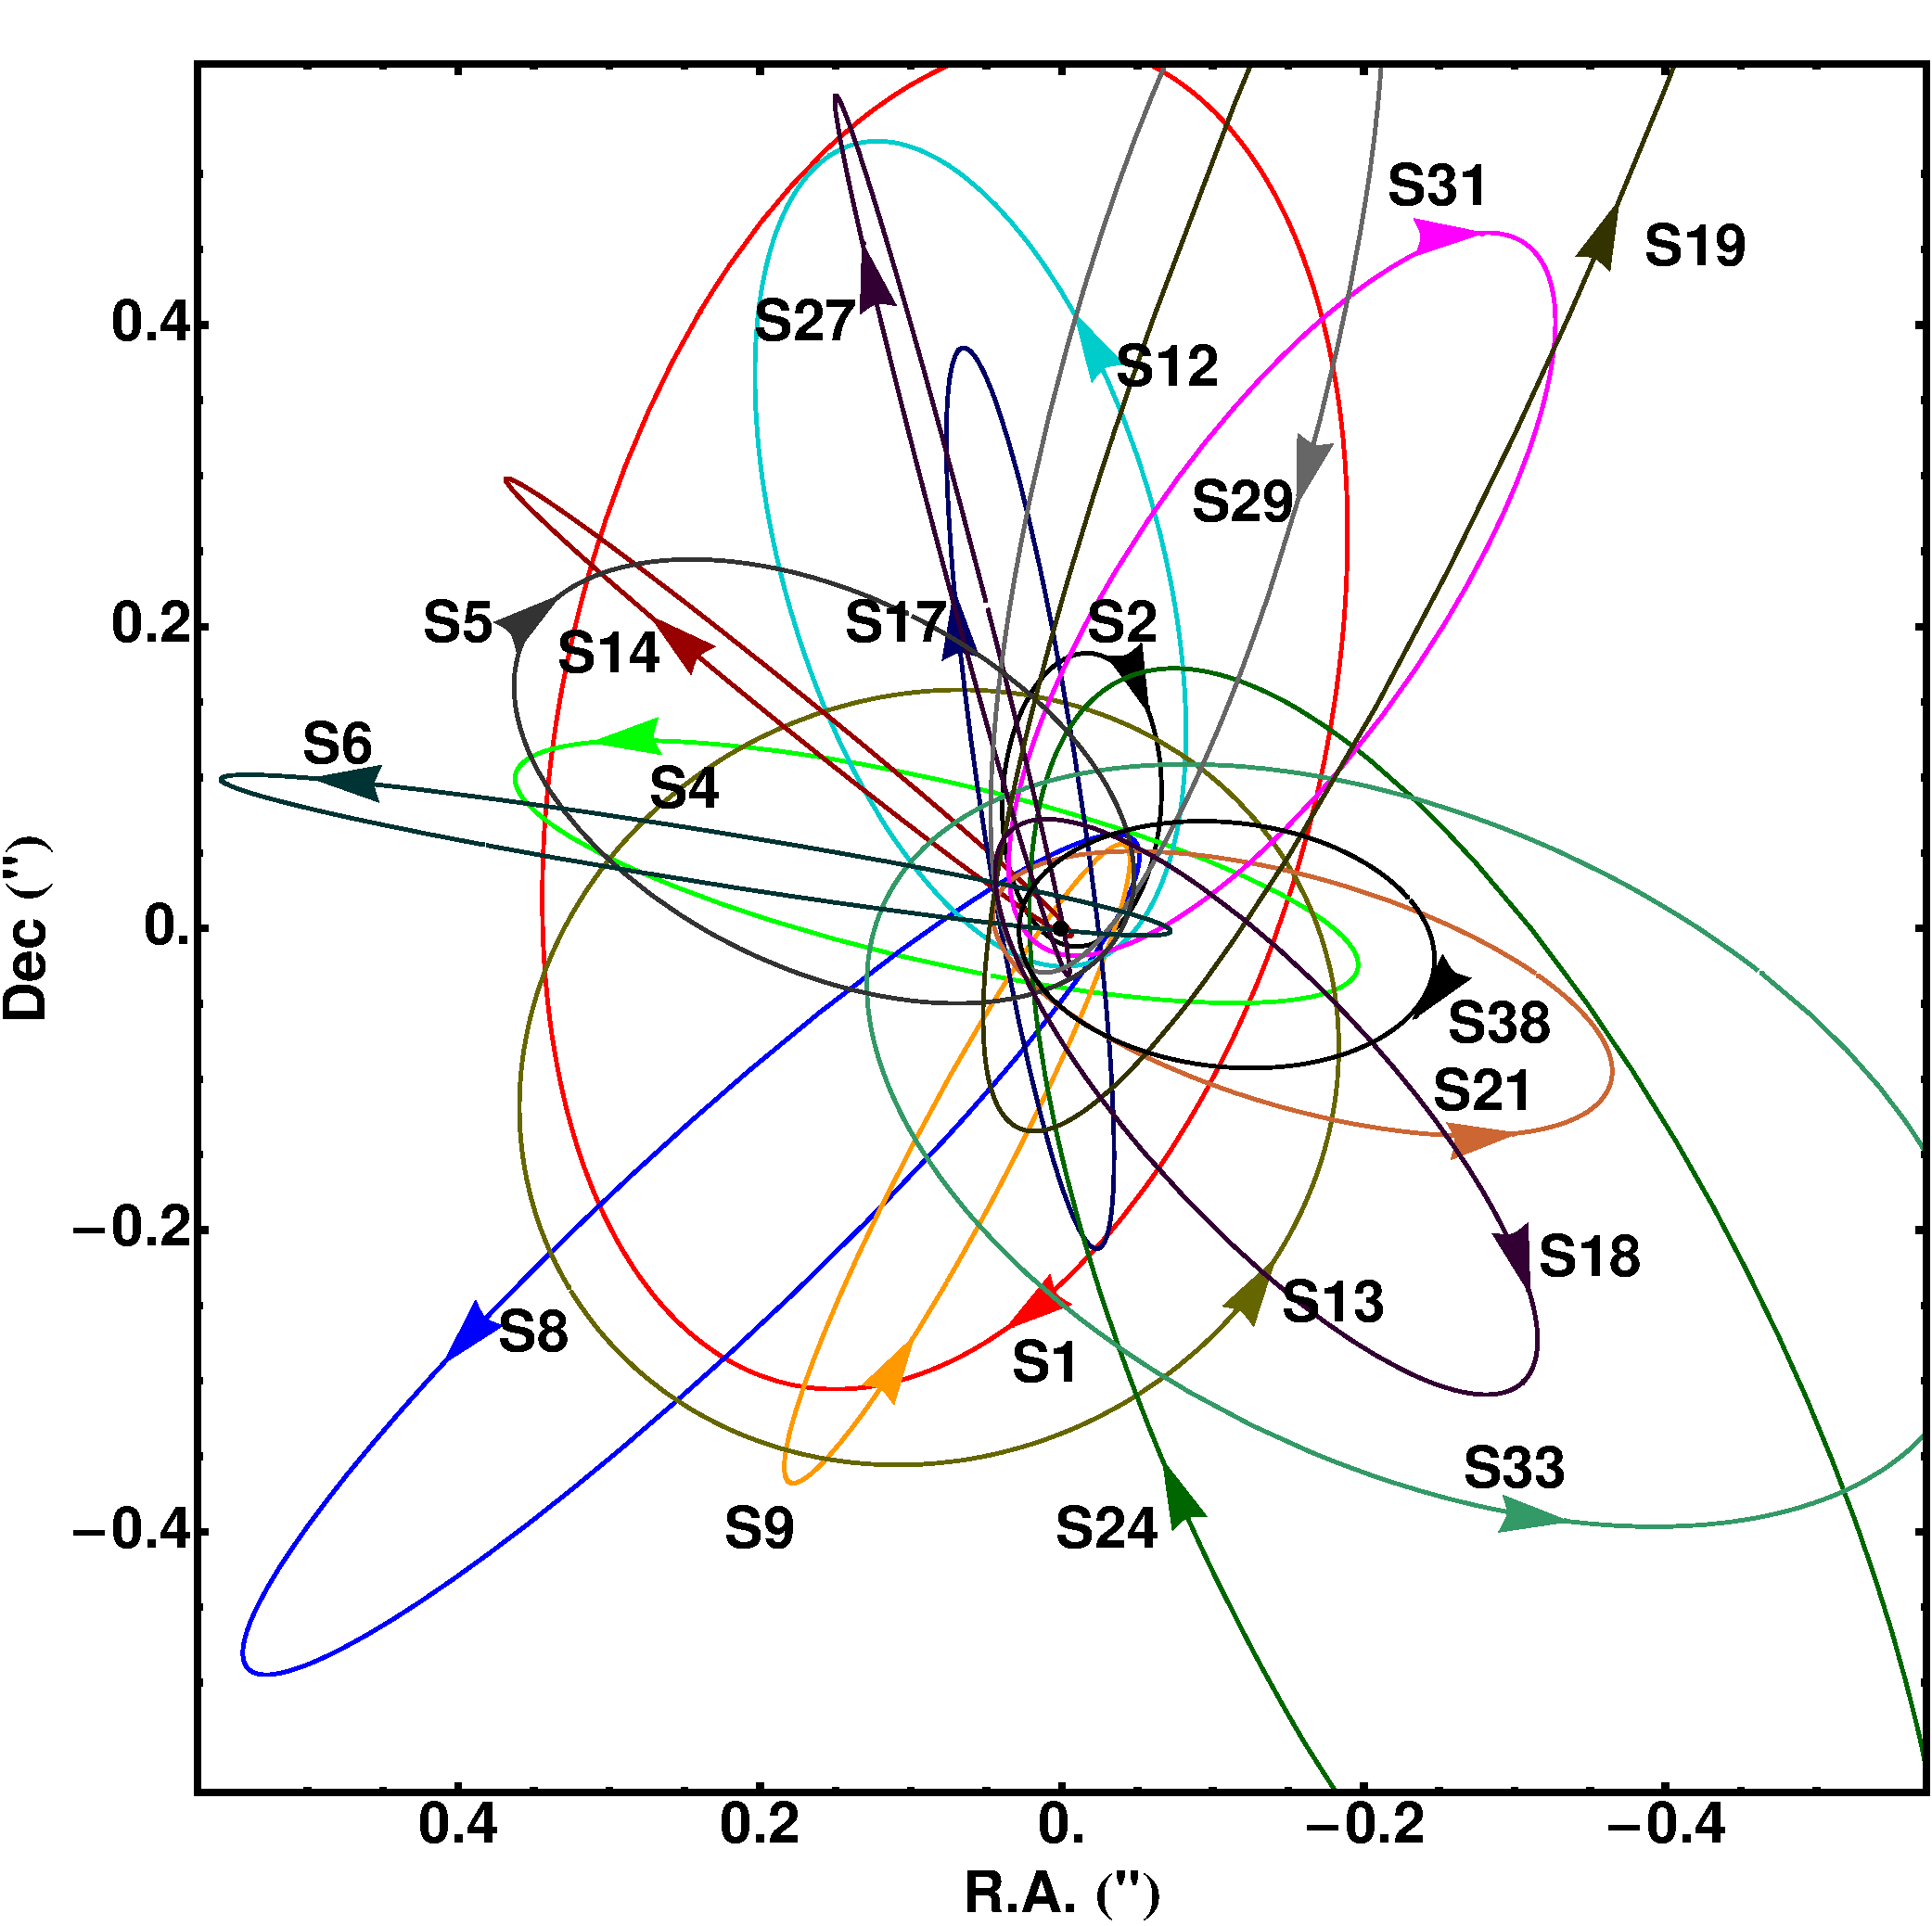
\includegraphics[width=7cm]{Immagini/orbite_sgra}
  \caption[Orbite di alcune delle stelle che intorno al buco nero
  Sgr~A*]{Rappresentazione delle orbite di alcune delle stelle che orbitano
    intorno al buco nero. La figura, tratta da \textcite{2009ApJ...692.1075G}, è
    centrata in Sgr~A*}
  \label{fig:orbite-sgra}
\end{figure}
Si suppone che la regione Sagittarius~A* (Sgr~A*), nel centro della nostra
galassia, sia sede di un buco nero supermassivo, cioè con una massa oltre $10^6$
volte più grande di quella del Sole. Intorno a questo buco nero orbitano
numerose stelle e le orbite di alcune di esse possono essere osservate nella
Figura~\ref{fig:orbite-sgra}. La stella più importante per i nostri scopi è S2
(chiamata a volte S0-2 e di massa circa \SI{15}{\solarmass}), poiché fra le
stelle che orbitano intorno al buco nero è quella che ha il più breve periodo di
rivoluzione, pari a circa $15$ anni, e fra le stelle di questa regione a breve
periodo è la più luminosa, quindi più facile da individuare. Le osservazioni
astronomiche di S2 sono cominciate nel 1992 e da pochi anni ha completato
un'intera rivoluzione a partire da quella data, quindi è una ricca fonte di
informazioni per lo studio del buco nero. L'orbita di S2 intorno al buco nero
può essere considerata con buona approssimazione kepleriana quindi possiamo
utilizzare la~\eqref{eq:terza-legge-keplero} per stimare la massa
$M_\textup{BH}$ del buco nero. \textcite{2008ApJ...689.1044G} hanno studiato il
moto di S2 ricavando i dati riportati nella
Tabella~\ref{tab:parametri-orbitali-S2}.
\begin{table}
  \centering
  \caption[Parametri orbitali della stella S2]{Parametri orbitali della stella
    S2. $R_0$ è la distanza dalla Terra, $P$ è il periodo di rivoluzione, $a$
    è il semiasse maggiore dell'orbita ed $e$ la sua eccentricità,
    $R_\textup{min}$ è la distanza di periapside e $M_{\textup{S}2}$ è la
    massa della stella}
  \label{tab:parametri-orbitali-S2}
  \begin{tabular}{lc}
    \toprule
    Grandezza & Valore \\
    \midrule
    $R_0$ & \SI{7.96}{\kilo\parsec} \\
    $P$ & \SI{15.86}{\year} \\
    $a$ & \SI{126.5}{\milli\arcsecond} \\
    $e$ & $0.8970$ \\
    $R_\textup{min}$ & \SI{0.535}{\milli\parsec} \\
    $M_{\textup{S}2}$ & circa \SI{15}{\solarmass} \\
    \bottomrule
  \end{tabular}
\end{table}
Il semiasse maggiore dell'orbita è espresso in millesimi di arcosecondo, questo
valore può essere convertito in parsec, conoscendo la distanza $R_0$ della Terra
dal corpo, con la seguente relazione
\begin{equation}
  a [\si{\parsec}] = \frac{a [\si{\arcsecond}] \cdot R_0 [\si{\parsec}] \cdot
    \pi}{3600 \cdot 180} = \SI{4.88e-3}{\parsec}.
\end{equation}
Poiché $M_\textup{BH}$ è sicuramente molto più grande di $M_{\textup{S}2}$
possiamo porre $M_\textup{T} \approx M_\textup{BH}$
nella~\ref{eq:terza-legge-keplero} e otteniamo
\begin{equation}
  M_\textup{BH} \approx M_\textup{T} = \frac{4\pi^2a^3}{GP^2} =
  \SI{4.06e6}{\solarmass}.
\end{equation}
In realtà quella calcolata non è esattamente la massa del buco nero ma tutta la
massa che, nel piano dell'orbita di S2, è contenuta nella circonferenza di
raggio $R_\textup{min}$ e centro nel fuoco. Metodi più elaborati per la stima
della massa del buco nero possono essere trovati in
\textcite{2008ApJ...689.1044G} e \textcite{2009ApJ...692.1075G}.

Gli astronomi continuano a studiare il moto di S2 poiché sperano di osservare
delle deviazioni dall'orbita puramente kepleriana previste dalla teoria della
relatività le quali permetterebbero di effettuare una diversa stima della massa
del buco nero.

\section{I pianeti extrasolari}
\label{sec:extrasolari}

In questo paragrafo vedremo come è possibile ottenere alcune proprietà dei
pianeti extrasolari studiando le eclissi delle stelle intorno a cui orbitano e
con cui costituiscono quindi un sistema binario, almeno in prima
approssimazione.

Vediamo sotto quali condizioni è possibile per un osservatore esterno vedere
un'eclissi della stella dietro al pianeta studiato. Per semplicità Assumiamo che
le orbite dei due corpi siano circolari, quindi $e \approx 0$, che questi siano
perfettamente sferici e che possano essere trascurati gli effetti dovuti
all'atmosfera. Con riferimento alla Figura % TODO: creare figura, scrivere
                                % didascalia che faccia riferimento al fatto che
                                % il piano in cui si svolgono le orbite dei due
                                % corpi è ortogonale al piano della figura e
                                % inserire riferimento nel testo
il corpo di massa $m_1$ è la stella, di raggio $R$, e quello di massa $m_2$ è il
pianeta, il cui raggio è $r$. La distanza reciproca fra i centri dei due corpi
vale $a$. Se indichiamo con $i \in \mathopen{[}0, \pi/2\mathclose{]}$ l'angolo
di inclinazione sotto il quale l'osservatore vede il sistema, l'angolo minimo
che permette all'osservatore di assistere a un'eclissi è quello rappresentato
nella figura, cioè con l'asse $x''$ passante per il centro della stella e
tangente alla superficie del pianeta. Dunque
\begin{equation}
  \cos(\pi/2 - i) = \frac{\sqrt{a^2 - r^2}}{a} = \sqrt{1 - \frac{r^2}{a^2}}.
\end{equation}
Generalmente si ha $a \gg R \gg r$, quindi $\cos(\pi/2 - i) \approx 1$, cioè
$i \approx \pi/2$.

Nella Figura % TODO: creare figura, scrivere didascalia descrittiva che faccia
             % riferimento anche alla curva di luminosità e inserire riferimento
è rappresentata una schematizzazione di un'eclissi della stella, nel caso in cui
$i = \pi/2$. L'osservatore è fisso davanti alla stella e vede il pianeta che le
passa davanti, in vari istanti. Quando il pianeta non copre la stella la
luminosità del sistema è massima, quando inizia a nasconderla parzialmente
(istante di \emph{ingresso iniziale}, $t_{\textup{ii}}$) la luminosità decresce
fino a raggiungere un minimo nell'istante in cui si trova completamente davanti
alla stella (\emph{ingresso finale}, $t_{\textup{if}}$). La luminosità rimane
minima per tutto il tempo in cui il pianeta si trova davanti alla stella,
successivamente aumenta quando il pianeta esce parzialmente dalla stella
(\emph{egresso iniziale}, $t_{\textup{ei}}$) e ritorna massima non appena il
pianeta non copre più la stella (\emph{egresso finale}, $t_{\textup{ef}}$). Gli
istanti fin qui definiti sono detti \emph{punti di contatto}. Esistono poi i
\emph{punti di mezzo ingresso} che sono quelli in cui la curva di luminosità
raggiunge il valore intermedio fra il massimo e il minimo. In particolare
abbiamo il \emph{mezzo ingresso iniziale} ($t_{\textup{mi}}$) quando la
luminosità sta diminuendo e il \emph{mezzo ingresso finale} ($t_{\textup{mf}}$)
quando la luminosità ricomincia ad aumentare. Definiamo la
\emph{durata dell'eclissi} $\Delta t$ come il tempo che intercorre fra
l'ingresso iniziale e l'egresso finale:
$\Delta t = t_{\textup{ef}} - t_{\textup{ii}}$. La velocità di rivoluzione del
pianeta intorno alla stella è $P/(2\pi a)$, avendo indicato con $P$ il periodo
di rivoluzione del pianeta intorno alla stella, e, sempre nell'approssimazione
$a \gg R \gg r$, lo spazio percorso dal pianeta fra gli istanti
$t_{\textup{ii}}$ e $t_{\textup{ef}}$ è $2(R + r)$. Allora la durata
dell'eclissi è
\begin{equation}
  \Delta t \approx \frac{P}{2\pi a}2(R + r) = \frac{P(R + r)}{\pi a}.
\end{equation}

Se l'angolo di inclinazione $i$ non vale esattamente $\pi/2$, anche, come
abbiamo visto, per poter osservare un'eclissi deve comunque aversi $i \approx
\pi/2$, l'osservatore non vede il pianeta passare esattamente davanti
all'equatore della stella ma leggermente più spostato, come nella Figura % TODO:
                                % inserire figura e riferimento.
. Per calcolare lo spostamento apparente del pianeta rispetto all'equatore si
può vedere la Figura. % TODO: inserire figura e riferimento (se riesci puoi
                      % mettere questa figura e la precedente insieme).
Da semplici calcoli trigonometrici si ricava che lo spostamento apparente vale
$a \cos i$. Le definizioni dei punti di contatto e di mezzo ingresso valgono
anche per questo caso. Osservando la Figura % TODO: inserire riferimento
                                % all'ultima figura
si ricava, con semplici ragionamenti trigonometrici, che lo spazio percorso dal
pianeta fra gli istanti $t_{\textup{ii}}$ e $t_{\textup{ef}}$ è $2(R + r)$ è
circa $2\sqrt{(R + r)^2 - a^2\cos^2 i}$, quindi la durata dell'eclissi in questo
caso è
\begin{equation}
  \Delta t \approx \frac{P}{2\pi a} 2\sqrt{(R + r)^2 - a^2\cos^2 i} =
  \frac{P}{\pi} \sqrt{\left(\frac{R + r}{a}\right)^2 - \cos^2 i}.
\end{equation}
Per $i = \pi/2$ si riottiene il risultato precedente.

\section{La funzione di massa. Sistemi binari X}
\label{sec:funzione-massa}

Vediamo ora un nuovo modo per stimare la massa di un corpo celeste sfruttando la
terza legge di Keplero. Sappiamo che
\begin{equation}
  \label{eq:terza-legge-keplero2}
  G(m_1 + m_2)  P^2 = 4\pi^2a^3,
\end{equation}
dove $a$ è il semiasse maggiore dell'ellisse descritta dalla particella
relativa. Per ragioni di similitudine, il rapporto $a_1/a$, con $a_1$ semiasse
maggiore dell'orbita descritta dal corpo di massa $m_1$, è uguale al rapporto
$\norm{\bm{r}_1/\bm{r}}$, cioè dalla~\eqref{eq:r1-nel-cdm}
\begin{equation}
  \label{eq:semiasse-m1}
  a_1 = \frac{\mu}{m_1}a = \frac{m_2}{m_1 + m_2}a.
\end{equation}
Quindi, sostituendo la~\eqref{eq:semiasse-m1}
nella~\eqref{eq:terza-legge-keplero2} abbiamo
\begin{equation}
  GP^2\frac{m_2^3}{(m_1 + m_2)^3} = 4\pi^2a_1^3.
\end{equation}
Nelle osservazioni spettroscopiche non possono essere misurati separatamente il
semiasse maggiore $a_1$ e l'angolo di inclinazione $i$, ma la proiezione di
$a_1$ nel piano del cielo data da $a_1\sin i$. Moltiplicando ambo i membri per
$\sin^3 i$ e portando al secondo membro tutte le quantità misurabili risulta
\begin{equation}
  \label{eq:valore-funzione-massa}
  \frac{(m_2\sin i)^3}{(m_1 + m_2)^2} = \frac{4\pi^2}{GP^2}(a_1\sin i)^3.
\end{equation}
Il primo membro dell'equazione prende il nome di \emph{funzione di massa} per il
corpo $1$
\begin{equation}
  f_1(m_1,m_2,i) = \frac{(m_2\sin i)^3}{(m_1 + m_2)^2}.
\end{equation}
Il valore della funzione di massa è noto quando si misurano il periodo orbitale
$P$ e il semiasse maggiore proiettato $a_1\sin i$. È possibile fare questo, in
particolare misurare $a_1\sin i$, solo nei sistemi visuali, quelli cioè in cui
entrambi i corpi che costituiscono sono visibili. Vedremo più avanti come si può
calcolare la funzione di massa negli altri casi. Ragionando in maniera analoga
per il corpo di massa $m_2$ possiamo definire la funzione di massa $f_2$
\begin{equation}
  f_2(m_1,m_2,i) \equiv \frac{(m_1\sin i)^3}{(m_1 + m_2)^2} =
  \frac{4\pi^2}{GP^2}(a_2\sin i)^3,
\end{equation}
con $a_2$ semiasse maggiore dell'ellisse descritta dal corpo di massa
$m_2$. Conoscendo solo le funzioni di massa non è possibile determinare
univocamente le due masse se l'angolo di inclinazione non è noto. Sarà quindi
necessaria un'altra equazione per poter fissare i valori di tutte e tre queste
grandezze. Tuttavia, dato un qualsiasi valore di $m_1$ e $i$, la funzione di
massa $f_1$ fornisce il minimo valore della massa $m_2$. Allo stesso modo, il
valore di $f_2$ è un limite inferiore per la massa del corpo $1$.

Utilizziamo la funzione di massa per stimare la massa di un corpo non visibile
che costituisce insieme alla stella variabile supergigante HD 226868 il sistema
binario
Cygnus-X1.\footnote{I dati riportati di seguito sono presi
  da~\textcite{melia:astrophysics}.} Poiché il corpo non emette nella banda
ottica sicuramente non è una stella. È noto che l'eccentricità del sistema è
molto piccola ($e \lesssim 0.02$), quindi possiamo considerare l'orbita
circolare. Misure basate sull'effetto Doppler forniscono la velocità orbitale
proiettata $v_1$ della stella e risulta $v_1 =
\SI{75}{\kilo\metre\per\second}$. Inoltre le variazioni periodiche del flusso
misurato della stella fornisce il periodo di rotazione $P =
\SI{5.6}{\day}$. Possiamo scrivere la velocità orbitale proiettata come
\begin{equation}
  \label{eq:velocità-proiettata}
  v_1 = \frac{2\pi}{P}a_1\sin i,
\end{equation}
con $a_1$ semiasse maggiore dell'orbita della stella. Inserendo
la~\eqref{eq:velocità-proiettata} nella~\eqref{eq:valore-funzione-massa} abbiamo
\begin{equation}
  f_1(m_1,m_2,i) \equiv \frac{(m_2\sin i)^3}{(m_1 + m_2)^2} = \frac{v_1^3P}{2\pi
    G}.
\end{equation}
Poiché per questo sistema si hanno delle eclissi l'angolo di inclinazione vale
$i \simeq \pi/2$, quindi $\sin \simeq 1$. Da osservazioni nella banda ottica si
è trovato
\begin{equation}
  f_1 = \SI{0.252(10)}{\solarmass}.
\end{equation}
Si stima che la stella abbia una massa $m_1 \gtrsim \SI{8.5}{\solarmass}$,
quindi la sua compagna ha una massa
\begin{equation}
  m_2 \gtrsim \SI{4}{\solarmass}.
\end{equation}
Poiché questo valore è maggiore del limite di Chandrasekhar % TODO: mettere un
                                % riferimento bibliografico.
$M_\textup{Ch} \simeq \SI{3}{\solarmass}$ per una stella di neutroni in
rotazione, dobbiamo concludere che il corpo non visibile del sistema Cygnus-X1 è
un buco nero.

%%% Local Variables:
%%% mode: latex
%%% TeX-master: "../tesi"
%%% End:


\appendix{}
\chapter{Programma per la soluzione dell'equazione di Keplero}
\label{cha:soluzione-keplero}

Di seguito è riportato il codice sorgente del programma usato per risolvere
l'equazione di Keplero con i metodi numeric di Newton~-~Raphson e dei
coefficienti di Bessel, illustrati nel
paragrafo~\ref{sec:soluzione-keplero}. Per calcolare i coefficienti di Bessel ho
utilizzato la GNU Scientific Library (GSL).\footnote{La GSL è software libero e
  il codice sorgente può essere scaricato e consultato da Internet all'indirizzo
  \url{http://www.gnu.org/software/gsl/}.} Anche la libreria per il C che ho
usato, Embedded GLIBC (EGLIBC),\footnote{La EGLIBC è software libero il codice
  sorgente può essere scaricato e consultato da Internet all'indirizzo
  \url{http://www.eglibc.org/}.} definisce una funzione per calcolare i
coefficienti di Bessel, ma la GSL è più efficiente. Il programma è suddiviso in
tre file: \verb|keplero.c| che contiene il \verb|main|, l'header
\verb|libreria.h| e la libreria \verb|libreria.c|. Per compilare il programma in
ambiente GNU/Linux ho usato i seguenti comandi da terminale
\begin{verbatim}
$ gcc -c -Wall -pedantic -lm -lgsl -lgslcblas libreria.c
$ gcc -Wall -pedantic -lm -lgsl -lgslcblas -o keplero \
  keplero.c libreria.o
\end{verbatim}
L'esecuzione del programma genera due file di testo, \verb|bessel.dat| e
\verb|newton.dat|, contenenti i risultati delle simulazioni effettuate con i due
diversi metodi.
% TODO: ho commentato l'inserimento del codice per accelerare i tempi di
% compilazione del documento, ricordarsi di decommentare nella versione finale!
% \lstinputlisting[language=C,caption={File \texttt{keplero.c}}]
% {programmi/keplero.c}
% \lstinputlisting[language=C,caption={File \texttt{libreria.h}},
% label={lst:lib.h}]{{programmi/libreria.h}}
% \lstinputlisting[language=C,caption={File \texttt{libreria.c}},
% label={lst:lib.c}]{{programmi/libreria.c}}

Qui riportiamo inoltre il codice dello script \verb|gnuplot| utilizzato per
ottenere le figure del paragrafo~\ref{sec:soluzione-keplero} a partire dai file
di output generati dall'esecuzione del programma. Per generare i grafici ho
utilizzato il seguente comando da terminale
\begin{verbatim}
$ gnuplot programmi/keplero.gnuplot
\end{verbatim}
che ho eseguito nella cartella superiore rispetto a quella in cui si trova lo
script \verb|keplero.gnuplot|.
\lstinputlisting[language=gnuplot,caption={File \texttt{keplero.gnuplot}}]
{programmi/keplero.gnuplot}

\clearpage{}
\chapter{Programma per la simulazione di un'eclissi}
\label{cha:simulazione-eclissi}

Riporto il codice sorgente del programma che ho scritto per effettuare la
simulazione di un'eclissi di una stella dietro a un pianeta, usando le
informazioni descritte nel paragrafo~\ref{sec:extrasolari}. Per calcolare le
posizioni della particella relativa e dei due corpi ho utilizzato le funzioni
presenti nella libreria riportata nei codici~\ref{lst:lib.h} e
\ref{lst:lib.c}. Il \verb|main| del programma è contenuto nel file
\verb|eclissi.c|. Per compilare il programma in ambiente GNU/Linux ho usato i
seguenti comandi da terminale
\begin{verbatim}
$ gcc -c -Wall -pedantic -lm -lgsl -lgslcblas libreria.c
$ gcc -Wall -pedantic -lm -lgsl -lgslcblas -o eclissi \
  eclissi.c libreria.o
\end{verbatim}
Eseguendo il programma si ottiene un file di testo, \verb|eclissi.dat|, con i
risultati della simulazione.
% TODO: ho commentato l'inserimento del codice per accelerare i tempi di
% compilazione del documento, ricordarsi di decommentare nella versione finale!
% \lstinputlisting[language=C,caption={File \texttt{eclissi.c}}]
% {programmi/eclissi.c}

Di seguito è riportato lo script \verb|gnuplot| utilizzato per produrre, con il
file generato dall'esecuzione del programma, le
figure~\ref{fig:sim-ecl-piano-cielo}, \ref{fig:sim-ecl-distanza-proiettata} e
\ref{fig:sim-ecl-flusso}. Per realizzare i grafici ho utilizzato il seguente
comando da terminale
\begin{verbatim}
$ gnuplot programmi/eclissi.gnuplot
\end{verbatim}
che ho eseguito nella cartella superiore rispetto a quella in cui si trova lo
script \verb|eclissi.gnuplot|.
\lstinputlisting[language=gnuplot,caption={File \texttt{eclissi.gnuplot}}]
{programmi/eclissi.gnuplot}

%%% Local Variables:
%%% mode: latex
%%% TeX-master: "../tesi"
%%% End:


\backmatter{}
\clearpage{}
\phantomsection{}
\addcontentsline{toc}{chapter}{Riferimenti bibliografici}
\printbibliography[title=Riferimenti bibliografici]

\end{document}
